\subsection{23. Classification}\label{classification}

\subsubsection{23.1 Introduction}\label{introduction}

The problem of predicting a discrete variable \(Y\) from another random
variable \(X\) is called \textbf{classfication}, \textbf{supervised
learning}, \textbf{discrimination} or \textbf{pattern recognition}.

In more detail, consider IID data \((X_1, Y_1), \dots, (X_n, Y_n)\)
where

\[ X_i = (X_{i1}, \dots, X_{id}) \in \mathcal{X} \subset \mathbb{R}^d \]

is a \(d\)-dimensional vector and \(Y_i\) takes values in some finite
set \(\mathcal{Y}\). A \textbf{classification rule} is a function \$h :
\mathcal{X} \rightarrow \mathcal{Y} \$. When we observe a new \(X\), we
predict \(Y\) to be \(h(X)\).

It is worth revisiting the vocabulary:

\begin{longtable}[]{@{}
  >{\raggedright\arraybackslash}p{(\columnwidth - 4\tabcolsep) * \real{0.1928}}
  >{\raggedright\arraybackslash}p{(\columnwidth - 4\tabcolsep) * \real{0.2530}}
  >{\raggedright\arraybackslash}p{(\columnwidth - 4\tabcolsep) * \real{0.5542}}@{}}
\toprule
\begin{minipage}[b]{\linewidth}\raggedright
Statistics
\end{minipage} & \begin{minipage}[b]{\linewidth}\raggedright
Computer Science
\end{minipage} & \begin{minipage}[b]{\linewidth}\raggedright
Meaning
\end{minipage} \\
\midrule
\endhead
classification & supervised learning & predicting a discrete \(Y\) from
\(X\) \\
data & training sample & \((X_1, Y_1), \dots, (X_n, Y_n)\) \\
covariates & features & the \(X_i\)'s \\
classifier & hypothesis & map
\(h: \mathcal{X} \rightarrow \mathcal{Y}\) \\
estimation & learning & finding a good classifier \\
\bottomrule
\end{longtable}

In most cases with this chapter, we deal with the case
\(\mathcal{Y} = \{ 0, 1 \}\).

\subsubsection{23.2 Error Rates and The Bayes Classifier}\label{error-rates-and-the-bayes-classifier}

The \textbf{true error rate} of a classifier is

\[ L(h) = \mathbb{P}( \{ h(X) \neq Y\} ) \]

and the \textbf{empirical error rate} or \textbf{training error rate} is

\[ \hat{L}_n(h) = \frac{1}{n} \sum_{i=1}^n I(h(X_i) \neq Y_i) \]

Consider the special case where \(\mathcal{Y} = \{0, 1\}\). Let

\[ r(x) = \frac{\pi f_1(x)}{\pi f_1(x) + (1 - \pi) f_0(x)} \]

where

\[ f_0(x) = f(x | Y = 0)
\quad \text{and} \quad
f_1(x) = f(x | Y = 1)\]

and \(\pi = \mathbb{P}(Y = 1)\).

The \textbf{Bayes classification rule} \(h^*\) is defined to be

\[
h^*(x) = \begin{cases}
1 & \text{if } r(x) > \frac{1}{2} \\
0 & \text{otherwise}
\end{cases}
\]

The set
\(\mathcal{D}(h) = \{ x : \mathbb{P}(Y = 1 | X = x) = \mathbb{P}(Y = 0 | X = x) \}\)
is called the \textbf{decision boundary}.

\textbf{Warning}: the Bayes rule has nothing to do with Bayesian
inference. We could estimate the Bayes rule using either frequentist or
Bayesian methods.

The Bayes rule may be written in several different forms:

\[
h^*(x) = \begin{cases}
1 & \text{if } \mathbb{P}(Y = 1 | X = x) > \mathbb{P}(Y = 0 | X  = x)\\
0 & \text{otherwise}
\end{cases}
\]

and

\[
h^*(x) = \begin{cases}
1 & \text{if } \pi f_1(x) > (1 - \pi) f_0(x) \\
0 & \text{otherwise}
\end{cases}
\]

\textbf{Theorem 23.5}. The Bayes rule is optimal, that is, if \(h\) is
any classification rule then \(L(h^*) \leq L(h)\).

The Bayes rule depends on unknown quantities so we need to use the data
to find some approximation to the Bayes rule. At the risk of
oversimplifying, there are three main approaches:

\begin{enumerate}
\def\labelenumi{\arabic{enumi}.}
\item
  \textbf{Empirical Risk Maximization}. Choose a set of classifiers
  \(\mathcal{H}\) and find \(\hat{h} \in \mathcal{H}\) that minimizes
  some estimate of \(L(h)\).
\item
  \textbf{Regression}. Find an estimate \(\hat{r}\) of the regression
  function \(r\) and define
\end{enumerate}

\[ 
\hat{h}(x) = \begin{cases}
1 & \text{if } \hat{r} > \frac{1}{2} \\
0 & \text{otherwise}
\end{cases}
\]

\begin{enumerate}[tightlist,label={\arabic*.},resume]
\item
  \textbf{Density Estimation}. Estimate \(f_0\) from the \(X_i\)'s for
  which \(Y_i = 0\), estimate \(f_1\) from the \(X_i\)'s for which
  \(Y_i = 1\), and let \(\hat{\pi} = n^{-1} \sum_{i=1}^n Y_i\). Define
\end{enumerate}

\[ \hat{r}(x) = \hat{\mathbb{P}}(Y = 1 | X = x) = \frac{\hat{\pi} \hat{f}_1(x)}{\hat{\pi} \hat{f}_1(x) + (1 - \hat{\pi}) \hat{f}_0(x)} \]

and

\[ 
\hat{h}(x) = \begin{cases}
1 & \text{if } \hat{r} > \frac{1}{2} \\
0 & \text{otherwise}
\end{cases}
\]

Now to generalize to the case where \(Y\) takes more than two values:

\textbf{Theorem 23.6}. Suppose that
\(Y \in \mathcal{Y} = \{ 1, \dots, K \}\). The optimal rule is

\[ h(x) = \text{argmax}_h \mathbb{P}(Y = k | X = x) = \text{argmax}_h \pi_k f_k(x) \]

where

\[ \mathbb{P}(Y = k | X = x) = \frac{f_k(x) \pi_k}{\sum_r f_r(x) \pi_r} \]

and \$ \pi\_r = \mathbb{P}(Y = r)\$, \(f_r(x) = f(x | Y = r)\).

\subsubsection{23.3 Gaussian and Linear Classifiers}\label{gaussian-and-linear-classifiers}

Perhaps the simplest approach to classification is to use the density
estimation strategy and assume a parametric model for the densities.
Suppose that \(\mathcal{Y} = \{ 0, 1 \}\) and that
\(f_0(x) = f(x | Y = 0)\) and \(f_1(x) = f(x | Y = 1)\) are both
multivariate Gaussians:

\[ f_k(x) = \frac{1}{(2\pi)^{d/2} | \Sigma_k |^{1/2}} \exp \left\{ -\frac{1}{2} (x - \mu_k)^T \Sigma_k^{-1} (x - \mu_k) \right\}, \quad k = 0, 1\]

Thus, \(X | Y = 0 \sim N(\mu_0, \Sigma_0)\) and
\(X | Y = 1 \sim N(\mu_1, \Sigma_1)\).

\textbf{Theorem 23.7}. If \(X | Y = 0 \sim N(\mu_0, \Sigma_0)\) and
\(X | Y = 1 \sim N(\mu_1, \Sigma_1)\), then the Bayes rule is

\[
h^*(x) = \begin{cases}
1 & \text{if } r_1^2 < r_0^2 + 2 \log \left( \frac{\pi_1}{\pi_0} \right) + \log \left( \frac{| \Sigma_0 | }{ | \Sigma_1| }
\right) \\
0 & \text{otherwise} 
\end{cases}
\]

where

\[ r_i^2 = (x - \mu_i)^T \Sigma_i^{-1}(x - \mu_i), \quad i = 1, 2 \]

is the \textbf{Manalahobis distance}. An equivalent way of expressing
Bayes' rule is

\[ h(x) = \text{argmax}_k \delta_k(x) \]

where

\[ \delta_k(x) = -\frac{1}{2} \log | \Sigma_k | - \frac{1}{2} (x - \mu_k)^T \Sigma_k^{-1} (x - \mu_k) + \log \pi_k \]

and \(|A|\) denotes the determinant of matrix \(A\).

The decision boundary of the above classifier is quadratic so this
procedure is often called \textbf{quadratic discriminant analysis
(QDA)}. In practice, we use sample estimates of
\(\pi, \mu_0, \mu_1, \Sigma_0, \Sigma_1\) in place of the true value,
namely:

\[
\begin{array}{cc}
\hat{\pi}_0 = \frac{1}{n} \sum_{i=1}^n (1 - Y_i) & \hat{\pi}_1 = \frac{1}{n} \sum_{i=1}^n Y_i \\
\hat{\mu}_0 = \frac{1}{n_0} \sum_{i: Y_i = 0} X_i & \hat{\mu}_1 = \frac{1}{n_0} \sum_{i: Y_i = 1} X_i \\
S_0 = \frac{1}{n_0} \sum_{i: Y_i = 0} (X_i - \hat{\mu}_0) (X_i - \hat{\mu}_0)^T & 
S_1 = \frac{1}{n_1} \sum_{i: Y_i = 1} (X_i - \hat{\mu}_1) (X_i - \hat{\mu}_1)^T
\end{array}
\]

where \(n_0 = \sum_i (1 - Y_i)\) and \(n_1 = \sum_i Y_i\) are the number
of \(Y_i\) variables equal to 0 or 1, respectively.

A simplification occurs if we assume \(\Sigma_0 = \Sigma_1 = \Sigma\).
In that case, the Bayes rule is

\[ h(x) = \text{argmax}_k \delta_k(x) \]

where now

\[ \delta_k(x) = x^T \Sigma^{-1} \mu_k - \frac{1}{2} \mu_k^T \Sigma^{-1} \mu_k + \log \pi_k \]

The parameters are estimated as before, except the MLE of \(\Sigma\) now
is

\[ S = \frac{n_0 S_0 + n_1 S_1}{n_0 + n_1} \]

The classification rule is

\[
h^*(x) = \begin{cases}
1 &\text{if } \delta_1(x) > \delta_0(x) \\
0 &\text{otherwise}
\end{cases}
\]

where

\[ \delta_j(x) = x^T S \hat{\mu}_j - \frac{1}{2} \hat{\mu}_j^T S^{-1} \hat{\mu}_j + \log \hat{\pi}_j \]

is called the \textbf{discriminant function}. The decision boundary \$
\{ x : \delta\_0(x) = \delta\_1(x) \}\$ is linear so this method is
called \textbf{linear discrimination analysis (LDA)}.

Now we generalize to the case where \(Y\) takes on more than two values.

\textbf{Theorem 23.9}. Suppose that \(Y \in \{ 1, \dots, K \}\). If
\(f_k(x) = f(x | Y = k)\) is Gaussian, the Bayes rule is

\[ h(x) = \text{argmax}_k \delta_k(x) \]

where

\[ \delta_k(x) = -\frac{1}{2} \log | \Sigma_k | - \frac{1}{2} (x - \mu_k)^T \Sigma_k^{-1} (x - \mu_k) + \log \pi_k \]

If the variances of the Gaussians are equal then

\[ \delta_k(x) = x^T \Sigma_{-1} \mu_k - \frac{1}{2} \mu_k^T \Sigma^{-1} \mu_k + \log \pi_k \]

We estimate \(\delta_k(x)\) by inserting estimates of \(\mu_k\),
\(\Sigma_k\), and \(\pi_k\).

There is another version of LDA due to Fisher. The idea is to first
reduce the dimension of the covariates to one dimension by projecting
the data onto a line. Algebraically, this means replacing the covariate
\(X = (X_1, \dots, X_d)\) with a linear combination
\(U = w^T X = \sum_{j=1}^d w_j X_j\). The goal is to choose the vector
\(w = (w_1, \dots, w_d)\) that ``best separates the data''. Then we
perform classification with the new covariate \(U\) instead of \(X\).

We need to define what we mean by separation of the groups. We would
like the two groups to have means that are far apart relative to their
spread. Let \(\mu_j\) denote the mean of \(X\) for \(Y = j\) and let
\(\Sigma\) be the variance matrix of \(X\). Then
\(\mathbb{E}(U | Y = j) = \mathbb{E}(w^T X | Y = j) = w^T \mu_j\) and
\(\mathbb{V}(U) = w^T \Sigma w\). Define the separation by

\[
\begin{align}
J(w) &= \frac{(\mathbb{E}(U | Y = 0) - \mathbb{E}(U | Y = 1))^2}{w^T \Sigma w} \\
&= \frac{(w^T \mu_0 - w^T \mu_1)^2}{w^T \Sigma w} \\
&= \frac{w^T (\mu_0 - \mu_1)(\mu_0 - \mu_1)^T w}{w^T \Sigma w}
\end{align}
\]

\emph{The quantity \(J\) arises in physics, where it is called the
Rayleight coefficient.}

We estimate \(J\) as follows. Let \(n_j = \sum_{i=1}^n I(Y_i = j)\) be
the number of observations in group \(j\), let
\(\overline{X}_j = n_j^{-1} \sum_{i: Y_i = j} X_j\) be the sample mean
vetor of \(X\)'s for group \(j\), and let \$S\_j = (n\_j - 1)\^{}\{-1\}
\sum\_\{i: Y\_i = j\} (X\_i - \overline{X}\_j)(X\_i -
\overline{X}\_j)\^{}T \$ be the sample covariance matrix in group \(j\).
Define

\[ \hat{J}(w) = \frac{w^T S_B w}{w^T S_W w} \]

where

\[ 
S_B = (\overline{X}_0 - \overline{X}_1) (\overline{X}_0 - \overline{X}_1)^T
\quad \text{and} \quad
S_W = \frac{(n_0 - 1) S_0 + (n_1 - 1) S_1}{(n_0 - 1) + (n_1 -1)}
\]

\textbf{Theorem 23.10}. The vector

\[ w = S_W^{-1}(\overline{X}_0 - \overline{X}_1) \]

is a minimizer of \(\hat{J}(w)\). We call

\[ U = w^T X = (\overline{X}_0 - \overline{X}_1)^T S_W^{-1} X \]

the \textbf{Fisher linear discriminant function}. The midpoint \(m\)
between \(\overline{X}_0\) and \(\overline{X}_1\) is

\[ m = \frac{1}{2} (\overline{X}_0 + \overline{X}_1) = \frac{1}{2}  (\overline{X}_0 - \overline{X}_1)^T S_B^{-1}  (\overline{X}_0 + \overline{X}_1)\]

Fisher's classification rule is

\[
h(x) = \begin{cases}
0 & \text{if } w^T X \geq m \\
1 & \text{if } w^T X < m
\end{cases}
= \begin{cases}
0 & \text{if } (\overline{X}_0 - \overline{X}_1)^T S_W^{-1}x \geq m \\
1 & \text{if } (\overline{X}_0 - \overline{X}_1)^T S_W^{-1}x < m
\end{cases}
\]

Fisher's rule is the same as the Bayes linear classifier when
\(\hat{\pi} = 1/2\).

\subsubsection{23.4 Linear Regression and Logistic Regression}\label{linear-regression-and-logistic-regression}

A more direct approach to classification is to estimate the regression
function \(r(x) = \mathbb{E}(Y | X = x)\) without bothering to estimate
the densities \(f_k\). For the rest of this section we will only
consider the case where \(\mathcal{Y} = \{ 0, 1 \}\). Thus,
\(r(x) = \mathbb{P}(Y = 1 | X = x)\) and once we have an estimate
\(\hat{r}\), we will use the classification rule

\[ 
h(x) = \begin{cases}
1 &\text{if } \hat{r}(x) > \frac{1}{2} \\
0 &\text{otherwise}
\end{cases} 
\]

The simplest regression is the linear regression model

\[ Y = r(x) + \epsilon = \beta_0 + \sum_{j=1}^d \beta_j X_j + \epsilon \]

where \(\mathbb{E}(\epsilon) = 0\). This model can't be correct since it
doesn't force \(Y \in \mathcal{Y}\). Nonetheless, it can sometimes lead
to a decent classifier.

Recall that the least square estimate of
\(\beta = (\beta_0, \beta_1, \dots, \beta_d)^T\) minimizes the residual
sum of squares

\[ \text{RSS}(\beta) = \sum_{i=1}^n \left( Y_i - \left( \beta_0  + \sum_{j=1}^d X_{ij} \beta_j \right) \right)^2 \]

Briefly reviewing this estimator: let

\[ 
X = \begin{bmatrix}
1 & X_{11} & \cdots & X_{1d} \\
1 & X_{21} & \cdots & X_{2d} \\
\vdots & \vdots & \ddots & \vdots \\
1 & X_{n1} & \cdots & X_{nd}
\end{bmatrix}
\quad \text{and} \quad
Y = (Y_1, \dots, Y_n)^T
\]

Then,

\[ \text{RSS}(\beta) = (Y - X \beta)^T (Y - X \beta) \]

and the model can be written as

\[ Y = X \beta + \epsilon \]

where \$ \epsilon = (\epsilon\_1, \dots, \epsilon\_n)\^{}T\$. The least
squares solution \(\hat{\beta}\) that minimizes RSS is given by

\[ \hat{\beta} = (X^T X)^{-1} X^T Y \]

and the predicted values are

\[ \hat{Y} = X \hat{\beta} \]

Now we can use \(h(x)\) to classify, by taking
\(\hat{r}(x) = \hat{\beta}_0 + \sum_k \hat{\beta}_k x_j\).

It seems sensible to use a regression model that takes into account that
\(Y \in \{ 0, 1 \}\). The most common method for doing so is
\textbf{logistic regression}. Recall that the model is

\[ r(x) = \mathbb{P}(Y = 1 | X = x) = \frac{\exp \left\{ \beta_0 + \sum_j \beta_j x_j \right\} }{1 + \exp \left\{ \beta_0 + \sum_j \beta_j x_j \right\} } \]

We may write this as

\[ \text{logit} \; \mathbb{P}(Y = 1 | X = x) = \beta_0 + \sum_j \beta_j x_j \]

where \(\text{logit}(a) = \log (a / (1 - a))\). Under this model, each
\(Y_i\) is a Bernoulli with success probability

\[ p_i(\beta) = \frac{\exp \left\{ \beta_0 + \sum_j \beta_j X_{ij} \right\} }{1 + \exp \left\{ \beta_0 + \sum_j \beta_j X_{ij} \right\} } \]

The likelihood function for the data set is

\[ \mathcal{L}(\beta) = \prod_{i=1}^n p_i(\beta)^{Y_i} (1 - p_i(\beta))^{1 - Y_i}\]

We obtain the MLE numerically.

We can get a better classifier by fitting a richer model. For example we
could fit

\[ \text{logit} \; \mathbb{P}(Y = 1 | X = x) = \beta_0 + \sum_j \beta_j x_j + \sum_{j, k} \beta_{jk} x_j x_k \]

More generally, we could add terms of up to order \(r\) for some integer
\(r\). Large values of \(r\) give a more complicated model which should
fit the data better. But there is a bias-variance tradeoff which we'll
discuss later.

The logistic regression can be easily extend to \(k\) groups but we
shall not give the details here.

\emph{(Student note: multiple treatments are easily found searching for
``multinomial logistic regression'')}

\subsubsection{23.5 Relationship Between Logistic Regression and LDA}\label{relationship-between-logistic-regression-and-lda}

LDA and logistic regression are almost the same thing.

If we assume each group is Gaussian with the same covariance matrix then

\[ 
\begin{align}
\log \left( \frac{\mathbb{P}(Y = 1 | X = x)}{\mathbb{P}(Y = 0 | X = x)} \right) 
&= \log \left( \frac{\pi_0}{\pi_1} \right) - \frac{1}{2} (\mu_0 + \mu_1)^T \Sigma^{-1} (\mu_1 - \mu_0) + x^T \Sigma^{-1}( \mu_1 - \mu_0) \\
&\equiv \alpha_0 + \alpha^T x
\end{align}
\]

On the other hand, the logistic model is, by assumption,

\[ \log \left( \frac{\mathbb{P}(Y = 1 | X = x)}{\mathbb{P}(Y = 0 | X = x)} \right) = \beta_0 + \beta^T x \]

These are the same model since they both lead to classification rules
that are linear in \(x\). The difference is in how we estimate the
parameters.

The joint density of a single observation is
\(f(x, y) = f(x | y) f(y) = f(y | x) f(x)\). In LDA we estimated the
whole distribution by estimating \(f(x | y)\) and \(f(y)\);
specifically, we estimated \(f_k(x) = f(x | Y = k)\),
\(\pi_k = f_Y(k)\). We maximized the likelihood

\[ \prod_i f(x_i, y_i) = \underbrace{\prod_i f(x_i | y_i)}_\text{Gaussian} \underbrace{ \prod_i f(y_i) }_\text{Bernoulli}\]

In logistic regression, we maximized the conditional likelihood
\(\prod_i f(y_i | x_i)\) but we ignored the second term \(f(x_i)\):

\[ \prod_i f(x_i, y_i) = \underbrace{\prod_i f(y_i | x_i)}_\text{logistic} \underbrace{ \prod_i f(x_i) }_\text{ignored}\]

Since classification requires only knowing \(f(y | x)\), we don't really
need to estimate the whole joint distribution. Logistic regression
leaves the marginal distribution \(f(x)\) unspecified so it is more
nonparametric than LDA.

To summarize: LDA and logistic regression both lead to a linear
classification rule. In LDA we estimate the whole joint distribution
\(f(x, y) = f(x | y) f(y)\). In logistic regression we only estimate
\(f(y | x)\) and we don't bother estimating \(f(x)\).

\subsubsection{23.6 Density Estimation and Naive Bayes}\label{density-estimation-and-naive-bayes}

Recall that the Bayes rule is \(h(x) = \text{argmax}_k \pi_k f_k(x)\).
If we can estimate \(\pi_k\) and \(f_k\) then we can estimate the Bayes
classification rule. Estimating \(\pi_k\) is easy, but what about
\(f_k\)? We did it previously by assuming \(f_k\) was Gaussian. Another
strategy is to estimate \(f_k\) with some nonparametric density
estimator \(\hat{f}_k\) such as a kernel estimator. But if
\(x = (x_1, \dots, x_d)\) is high dimensional, nonparametric density
estimation is not very reliable. The problem is ameliorated if we assume
that \(X_1, \dots, X_d\) are independent, for then
\(f_k(x_1, \dots, x_d) = \prod_{j=1}^d f_{kj}(x_j)\). This reduces the
problem to \(d\) one-dimensional density estimation problems, within
each of the \(k\) groups. The resulting classifier is called the
\textbf{naive Bayes classifier}. The assumption that the components of
\(X\) are independent is usually wrong yet the resulting classifier
might still be accurate.

\textbf{Naive Bayes Classifier}

\begin{enumerate}
\def\labelenumi{\arabic{enumi}.}
\item
  For each group \(k\), compute an estimate \(\hat{f}_{kj}\) of the
  density \(f_{kj}\) for \(X_j\), using the data for which \(Y_i = k\).
\item
  Let
\end{enumerate}

\[ \hat{f}_k(x) = \hat{f}_k(x_1, \dots, x_d) = \prod_{j=1}^d \hat{f}_{kj}(x_j) \]

\begin{enumerate}[tightlist,label={\arabic*.},resume]
\item
  Let
\end{enumerate}

\[ \hat{\pi}_k = \frac{1}{n} \sum_{i=1}^n I(Y_i = k) \]

where \(I(t) = 1\) if \(t\) and \(I(t) = 0\) otherwise.

\begin{enumerate}[tightlist,label={\arabic*.},resume]
\item
  Let
\end{enumerate}

\[ h(x) = \text{argmax}_k \hat{\pi}_k \hat{f}_k(x) \]

The naive Bayes classifier is especially popular when \(x\) is high
dimensional and discrete. In that case, \(\hat{f}_{kj}(x_k)\) is
especially simple.

\subsubsection{23.7 Trees}\label{trees}

Trees are classification methods that partition the covariate space
\(\mathcal{X}\) into disjoint pieces and then classify the observations
according to which partition element they fall in. As the name implies,
the classifier can be represented as a tree.

Here is how a tree is constructed. For simplicity, we focus on the case
where \(\mathcal{Y} = \{ 0, 1 \}\). First, suppose there is a single
covariate \(X\). We choose a split point \(t\) that divides the real
line into two sets, \(A_1 = (-\infty, t]\) and \(A_2 = (t, \infty)\).
Let \(\hat{p}_s(j)\) be the proportion of observations in \(A_s\) such
that \(Y_i = j\):

\[ \hat{p}_s(j) = \frac{\sum_{i=1}^n I(Y_i = j, X_i \in A_s)}{\sum_{i=1}^n I(X_i \in A_s)} \]

for \(s = 1, 2\) and \(j = 0, 1\). The \textbf{impurity} of the split
\(t\) is defined to be

\[ I(t) = \sum_{s=1}^2 \gamma_s \]

where

\[ \gamma_s = 1 - \sum_{j=0}^1 \hat{p}_s(j)^2 \]

This measure of impurity is known as the \textbf{Gini index}. If a
partition element \(A_s\) contains all 0s or all 1s, then
\(\gamma_s = 0\). Otherwise, \(\gamma_s > 0\). We choose the split point
\(t\) to minimize the impurity. (Other indices of impurity may be used
besides the Gini index.)

When there are several covariates, we choose whatever covariate and
split that leads to the lowest impurity. This process is continued until
some stopping criteria is met. For example, we might stop when every
partition element has fewer than \(n_0\) data points, where \(n_0\) is
some fixed number. The bottom nodes of the tree are called
\textbf{leaves}. Each leaf is assigned a 0 or 1 depending on whether
there are more data points with \(Y = 0\) or \(Y = 1\) in the partition
element.

This procedure is easily generalized to the multiclass case,
\(\mathcal{Y} = \{ 1, \dots, K \}\). We simply define the impurity by

\[ \gamma_s = 1 - \sum_{j=1}^K \hat{p}_s(j)^2 \]

where \(\hat{p}_s(j)\) is the proportion of observations in the
partition element for which \(Y = j\).

Our description of how to build trees is incomplete. If we keep
splitting until there are few cases in each leaf of the tree, we are
likely to overfit the data. We should choose the complexity of the tree
in such a way that the estimated true error rate is low. In the next
section, we discuss estimation of the error rate.

\subsubsection{23.8 Assessing Error Rates and Choosing a Good Classifier}\label{assessing-error-rates-and-choosing-a-good-classifier}

We would like to have a classifier \(h\) with a low true error rate
\(L(h)\). Usually, we can't use the training error rate \(\hat{L}_n(h)\)
as an estimate of the true error rate because it is biased downward.

There are many ways to estimate the error rate. We'll consider two:
\textbf{cross-validation} and \textbf{probability inequalities}.

\paragraph{Cross-validation}\label{cross-validation}

The basic idea of cross-validation is to leave out some of the data when
fitting a model. The simplest version involves randomly splitting the
data into two pieces: the \textbf{training set \(\mathcal{T}\)} and the
\textbf{validation set \(\mathcal{V}\)}. Often, about 10 percent of the
data might be set aside as the validation set. The classifier \(h\) is
constructed from the training set. We then estimate the error by

\[ \hat{L}(h) = \frac{1}{m} \sum_{X_i \in \mathcal{V}} I(h(X_i) \neq Y_i) \]

where \(m\) is the size of the validation set.

Another approach to cross-validation is \textbf{K-fold cross-validation}
which is obtained as follows:

\textbf{K-fold cross-validation}

\begin{enumerate}
\def\labelenumi{\arabic{enumi}.}
\item
  Randomly divide the data into \(K\) chunks of approximately equal
  size. A common choice is \(K = 10\).
\item
  For \(k = 1\) to \(K\) do the following:
\end{enumerate}

\begin{enumerate}
\def\labelenumi{(\alph{enumi})}
\item
  Delete chunk \(k\) from the data.
\item
  Compute the classifier \(\hat{h}_{(k)}\) from the rest of the data.
\item
  Use \(\hat{h}_{(k)}\) to predict the data in chunk \(k\). Let
  \(\hat{L}_{(k)}\) denote the observed error rate.
\end{enumerate}

\begin{enumerate}[tightlist,label={\arabic*.},resume]
\item
  Let
\end{enumerate}

\[ \hat{L}(h) = \frac{1}{K} \sum_{k=1}^K \hat{L}_{(k)} \]

Cross-validation can be applied to any classification method. To apply
it to trees, one begins by fitting an initial tree. Smaller trees are
obtained by pruning tree. We can do this for trees of various sizes,
where size refers to the number of terminal nodes on the tree.
Cross-validation is then used to estimate error rate as a function of
tree size.

\paragraph{Probability Inequalities}\label{probability-inequalities}

Another approach to estimating the error rate is to find a confidence
interval for \(\hat{L}_n(h)\) using probability inequalities. This
method is useful in the context of \textbf{empirical risk estimation}.

Let \(\mathcal{H}\) be a set of classifiers, for example, all linear
classifiers. Empirical risk minimization means choosing the classifier
\(\hat{h} \in \mathcal{H}\) to minimize the training error
\(\hat{L}_n(h)\), also called the empirical risk. Thus,

\[ \hat{h} = \text{argmin}_{h \in \mathcal{H}} \hat{L}_n(h) 
= \text{argmin}_{h \in \mathcal{H}} \left( \frac{1}{n} \sum_i I(h(X_i) \neq Y_i) \right) \]

Typically, \(\hat{L}_n(\hat{h})\) underestimates the true error rate
\(L(\hat{h})\) because \(\hat{h}\) was chosen to minimize
\(\hat{L}_n(\hat{h})\). Our goal is to assess how much underestimation
is taking place. Our main tool for this analysis is \textbf{Hoeffding's
inequality}. Recall that if
\(X_1, \dots, X_n \sim \text{Bernoulli}(p)\), then, for any
\(\epsilon > 0\),

\[ \mathbb{P}(|\hat{p} - p| > \epsilon) \leq 2 e^{ -2 n \epsilon^2 } \]

where \(\hat{p} = n^{-1} \sum_{i=1}^n X_i\).

First, suppose that \(\mathcal{H} = \{ h_1, \dots, h_m \}\) consists of
finitely many classifiers. For any fixed \(h\), \(\hat{L}_n(h)\)
converges in almost surely to \(L(h)\) by the law of large numbers. We
will now establish a stronger result.

\textbf{Theorem 23.16 (Uniform Convergence)}. Assume \(\mathcal{H}\) is
finite and has \(m\) elements. Then,

\[ \mathbb{P} \left( \max_{h \in \mathcal{H}} |\hat{L}_n(h) - L(h) | > \epsilon \right) \leq 2 m e^{-2 n \epsilon^2} \]

\textbf{Proof}. We will use Hoeffding's inequality and we will also use
the fact that if \(A_1, \dots, A_m\) is a set of events then
\(\mathbb{P}(\bigcup_{i=1}^m A_i) \leq \sum_{i=1}^m \mathbb{P}(A_i)\).
Now,

\[
\begin{align}
\mathbb{P} \left( \max_{h \in \mathcal{H}} |\hat{L}_n(h) - L(h) | > \epsilon \right)
&= \mathbb{P} \left( \bigcup_{h \in \mathcal{H}} |\hat{L}_n(h) - L(h) | > \epsilon \right) \\
& \leq \sum_{h \in \mathcal{H}} \mathbb{P} \left( |\hat{L}_n(h) - L(h) | > \epsilon \right) \\
& \leq \sum_{h \in \mathcal{H}} 2 e^{-2 n \epsilon^2} = 2 m e^{-2 n \epsilon^2}
\end{align}
\]

\textbf{Theorem 23.17}. Let

\[ \epsilon = \sqrt{\frac{2}{n} \log \left( \frac{2m}{\alpha} \right) } \]

Then \(\hat{L}_n(\hat{h}) \pm \epsilon\) is a \(1 - \alpha\) confidence
interval for \(L(\hat{h})\).

\textbf{Proof}. This follows from the fact that

\[
\mathbb{P}(|\hat{L}_n(\hat{h}) - L(\hat{h})| > \epsilon) 
\leq \mathbb{P}( \max_{h \in \mathcal{H}} |\hat{L}_n(h) - L(h) | > \epsilon )
\leq 2 m e^{-2 n \epsilon^2} = \alpha
\]

When \(\mathcal{H}\) is large the confidence interval for \(L(\hat{h})\)
is large. The more functions there are in \(\mathcal{H}\) the more
likely it is we have ``overfit'' which we compensate for by having a
larger confidence interval.

In practice, we usually use sets \(\mathcal{H}\) that are infinite, such
as the set of linear classifiers. To extend our analysis to these cases
we want to be able to say something like

\[ \mathbb{P} \left( \sup_{h \in \mathcal{H}} |\hat{L}_n(h) - L(h) | > \epsilon \right) \leq \text{something not too big} \]

All the other results followed from this inequality. One way to develop
such a generalization is by way of the \textbf{Vapnik-Chervonenkis} or
\textbf{VC dimension}. We now consider the main ideas in VC theory.

Let \(\mathcal{A}\) be a class of sets. Given a finite set
\(F = \{ x_1, \dots, x_n \}\) let

\[ N_\mathcal{A}(F) = \# \Big\{ F \cap A : A \in \mathcal{A} \Big\} \]

be the number of subsets F ``picked out'' by \(\mathcal{A}\). Here
\(\#(B)\) denotes the number of elements of set \(B\). The
\textbf{shatter coefficient} is defined by

\[ s(\mathcal{A}, n) = \max_{F \in \mathcal{F}_n} N_\mathcal{A}(F) \]

where \(\mathcal{F}_n\) consists of all finite sets of size \(n\). Now
let \(X_1, \dots, X_n \sim \mathbb{P}\) and let

\[ \mathbb{P}_n(A) = \frac{1}{n} \sum_i I(X_i \in A) \]

denote the empirical probability measure. The following remarkable
theorem bounds the distance between \(\mathbb{P}\) and \(\mathbb{P}_n\).

\textbf{Theorem 23.18 (Vapnik and Chervonenkis (1971))}. For any
\(\mathbb{P}\), \(n\), and \(\epsilon > 0\),

\[ \mathbb{P} \left\{ \sup_{A \in \mathcal{A}} | \mathbb{P}_n(A) - \mathbb{P}(A) | > \epsilon \right\} \leq 8 s(\mathcal{A}, n) e^{-n \epsilon^2 / 32} \]

The proof, though very elegant, is long and we omit it. If
\(\mathcal{H}\) is a set of classifiers, define \(\mathcal{A}\) to be
the class of sets of the form \(\{ x : h(x) = 1 \}\). Then we define
\(s(\mathcal{H}, n) = s(\mathcal{A}, n)\).

\textbf{Theorem 23.19}.

\[ \mathbb{P} \left\{ \sup_{h \in \mathcal{H}} | \hat{L}_n(h) - L(h) | > \epsilon \right\} \leq 8 s(\mathcal{H}, n) e^{-n \epsilon^2 / 32} \]

A \(1 - \alpha\) confidence interval for \(L(\hat{h})\) is
\(\hat{L}_n(\hat{h}) \pm \epsilon_n\) where

\[ \epsilon_n^2 = \frac{32}{n} \log \left( \frac{8 s(\mathcal{H}, n)}{\alpha} \right) \]

These theorems are only useful if the shatter coefficients do not grow
too quickly with \(n\). This is where the VC dimension enters.

The \textbf{VC (Vapnik-Chervonenkis) dimension} of a class of sets
\(\mathcal{A}\) is defined as follows. If \(s(\mathcal{A}, n) = 2^n\)
for all \(n\) set \(\text{VC}(\mathcal{A}) = \infty\). Otherwise, define
\(\text{VC}(\mathcal{A})\) to be the largest \(k\) for which
\(s(\mathcal{A}, n) = 2^k\).

Thus, the VC-dimension is the size of the largest finite set \(F\) that
can be \textbf{shattered by \(\mathcal{A}\)}, meaning that
\(\mathcal{A}\) picks out each subset of \(F\). If \(\mathcal{H}\) is a
set of classifiers we define
\(\text{VC}(\mathcal{H}) = \text{VC}(\mathcal{A})\) where
\(\mathcal{A}\) is the class of sets of the form \(\{ x : h(x) = 1 \}\)
as \(h\) varies in \(\mathcal{H}\). The following theorem shows that if
\(\mathcal{A}\) has finite VC-dimension then the shatter coefficients
grow as a polynomial in \(n\).

\textbf{Theorem 23.21}. If \(\mathcal{A}\) has finite VC-dimension
\(v\), then

\[ s(\mathcal{A}, n) \leq n^v + 1 \]

\textbf{Theorem 23.26}. Let \(x\) have dimension \(d\) and let
\(\mathcal{H}\) be the set of linear classifiers. The VC dimension of
\(\mathcal{H}\) is \(d + 1\). Hence, a \(1 - \alpha\) confidence
interval for the true error rate is \(\hat{L}(\hat{h}) \pm \epsilon\)
where

\[ \epsilon_n^2 = \frac{32}{n} \log \left( \frac{8 (n^{d + 1} + 1)}{\alpha} \right) \]

\subsubsection{23.9 Support Vector Machines}\label{support-vector-machines}

In this section we consider a class of linear classifiers called
\textbf{support vector machines}. Throughout this section, we assume
that \(Y\) is binary. It will be convenient to label the outcomes as
\(+1\) and \(-1\) instead of \(0\) and \(1\). A linear classifier can
then be written as

\[ h(x) = \text{sign}( H(x) ) \]

where \(x = (x_1, \dots, x_d)\),

\[ H(x) = a_0 + \sum_{i=1}^d a_i x_i \]

and

\[ \text{sign}(z) = \begin{cases}
-1 &\text{if } z < 0 \\
0  &\text{if } z = 0 \\
1  &\text{if } z > 0
\end{cases}\]

First, suppose that the data are \textbf{linearly separable}, that is,
there exists a hyperplane that perfectly separates the two classes.

\textbf{Lemma 23.27}. The data can be separated by some hyperplane if
and only if there exists a hyperplane \$H(x) = a\_0 + \sum\_\{i=1\}\^{}d
a\_i x\_i \$ such that

\[ Y_i H(x_i) \geq 1, \quad i = 1, \dots, n \]

\textbf{Proof}. Suppose that the data can be separated by a hyperplane
\(W(x) = b_0 + \sum_{i=1}^d b_i x_i\). It follows that there exists some
constant \(c\) such that \(Y_i = 1\) implies\(W(X_i) \geq c\) and
\(Y_i = -1\) implies \(W(X_i) \leq -c\). Therefore,
\(Y_i W(X_i) \geq c\) for all i. Let \(H(x) = a_0 + \sum_{i=1} a_i x_i\)
where \(a_i = b_i / c\). Then \(Y_i H(X_i) \geq 1\) for all \(i\). The
reverse direction is straightforward.

In the separable case, there will be many separating hyperplanes.
Intuitively, it seems reasonable to choose the hyperplane ``furthest''
from the data in the sense that it separates the +1s and -1s and
maximizes the distance to the closest point. This hyperplane is called
the \textbf{maximum margin hyperplane}. The margin is the distance from
the hyperplane to the nearest point. Points on the boundary of the
margin are called \textbf{support vectors}.

\textbf{Theorem 23.28}. The hyperplane
\(\hat{H}(x) = \hat{a}_0 + \sum_{i=1}^d \hat{a}_i x_i\) that separates
the data and maximizes the margin is given by minimizing
\((1/2) \sum_{j=1}^d b_j^2\) subject to \(Y_i H(x_i) \geq 1\).

It turns out that this problem can be recast as a quadratic programming
problem. Recall that \(\langle X_i, X_k \rangle = X_i^T X_k\) is the
inner product of \(X_i\) and \(X_k\).

\textbf{Theorem 23.29}. Let
\(\hat{H}(x) = \hat{a}_0 + \sum_{i=1}^d \hat{a}_i x_i\) denote the
optimal (largest margin) hyperplane. Then, for \(j = 1, \dots, d\),

\[ \hat{a}_j = \sum_{i=1}^n \hat{\alpha}_i Y_i X_j(i) \]

where \(X_j(i)\) is the value of the covariate \(X_j\) for the \(i\)-th
data point, and
\(\hat{\alpha} = (\hat{\alpha}_1, \dots, \hat{\alpha}_n)\) is the vector
that maximizes

\[ \sum_{i=1}^n \alpha_i - \frac{1}{2} \sum_{i=1}^n \sum_{k=1}^n \alpha_i \alpha_j Y_i Y_k \langle X_i, X_k \rangle \]

subject to

\[ \alpha_i \geq 0 \]

and

\[ 0 = \sum_i \alpha_i Y_i \]

The points \(X_i\) for which \(\hat{\alpha}_i \neq 0\) are called
\textbf{support vectors}. \(\hat{\alpha}_0\) can be found by solving

\[ \hat{\alpha_i}(Y_i (X_i^T \hat{\alpha} + \hat{\beta}_0)) = 0\]

for any support point \(X_i\). \(\hat{H}\) may be written as

\[ \hat{H}(x) = \hat{a}_0 + \sum_{i=1}^n \hat{\alpha}_i Y_i \langle x, X_i \rangle \]

There are many software packages that will solve this problem quickly.
If there is no perfect linear classifier, then one allows overlap
between the groups by replacing the condition \(Y_i H(x_i) \geq 1\) with

\[ Y_i H(x_i) \geq 1 - \xi_i,
\quad \xi_i \geq 0,
\quad i = 1, \dots, n
\]

The variables \(\xi_1, \dots, \xi_n\) are called \textbf{slack
variables}.

We now maximize
\(\sum_{i=1}^n \alpha_i - \frac{1}{2} \sum_{i=1}^n \sum_{k=1}^n \alpha_i \alpha_j Y_i Y_k \langle X_i, X_k \rangle\)
subject to

\[ 0 \leq \xi_i \leq c, \quad i = 1, \dots, n \]

and

\[ \sum_{i=1}^n \alpha_i Y_i = 0 \]

The constant \(c\) is a tuning parameter that controls the amount of
overlap.

\subsubsection{23.10 Kernelization}\label{kernelization}

There is a trick for improving a computationally simpler classifier
\(h\) called \textbf{kernelization}. The idea is to map the covariate
\(X\) -- which takes values in \(\mathcal{X}\) -- into a higher
dimensional space \(\mathcal{Z}\) and apply the classifier in the bigger
space \(Z\). This can yield a more flexible classifier while retaining
computational complexity.

The standard example of this is illustrated in the figure below. Let the
covariate be \(x = (x_1, x_2)\). The \(Y_i\)'s can be separated into two
groups using an ellipse. Define a mapping \(\phi\) by

\[ z = (z_1, z_2, z_3) = \phi(x) = (x_1^2, \sqrt{2} x_1 x_2, x_2^2) \]

This \(\phi\) maps \(\mathcal{X} = \mathbb{R}^2\) into
\(\mathcal{Z} = \mathbb{R}^3\). In the higher dimensional space
\(\mathcal{Z}\), the \(Y_i\)'s are separable by a linear decision
boundary. In other words, a linear classifier in a higher dimensional
space corresponds to a non-linear classifier in the original space.

\begin{python}
import numpy as np


# Fixing random state for reproducibility
np.random.seed(0)

# Generate data
X = np.random.uniform(low=-1, high=1, size=(2, 200))

def true_classifier(xx):
    return xx[0]**2 + 2 * xx[1]**2 <= 1

indexes = true_classifier(X)
A = X.T[indexes].T
B = X.T[~indexes].T

def phi(X):
    xx, yy = X[0].reshape(-1, 1), X[1].reshape(-1, 1)
    return np.concatenate([xx**2, np.sqrt(2) * xx * yy, yy**2], axis=1).T

phi_A, phi_B = phi(A), phi(B)
\end{python}

\begin{python}
import matplotlib.pyplot as plt
from matplotlib.patches import Ellipse
from mpl_toolkits.mplot3d import Axes3D  # Registers 3D projection

fig = plt.figure(figsize=(15, 8))
ax = plt.subplot(1, 2, 1)

ax.scatter(A[0], A[1], color='C0', marker='x')
ax.scatter(B[0], B[1], color='C1', marker='x')
ellipse = Ellipse(xy=[0,0], width=2, height=np.sqrt(2), angle=0,
              edgecolor='C0', lw=4, facecolor='none')
ax.add_patch(ellipse)
ax.set_xlabel(r'$x_1$')
ax.set_ylabel(r'$x_2$')

ax = plt.subplot(1, 2, 2, projection='3d')

ax.scatter(phi_A[0], phi_A[1], phi_A[2], marker='x')
ax.scatter(phi_B[0], phi_B[1], phi_B[2], marker='x')

xx, yy = np.meshgrid(np.arange(0, 1, step=0.1), np.arange(-1, 1, step=0.1))
zz = (1 - xx) / 2

ax.plot_surface(xx, yy, zz, alpha=0.2)

ax.set_xlabel(r'$x_1^2$')
ax.set_ylabel(r'$\sqrt{2} x_1 x_2$')
ax.set_zlabel(r'$x_2^2$')

plt.show()
\end{python}

\begin{figure}[H]
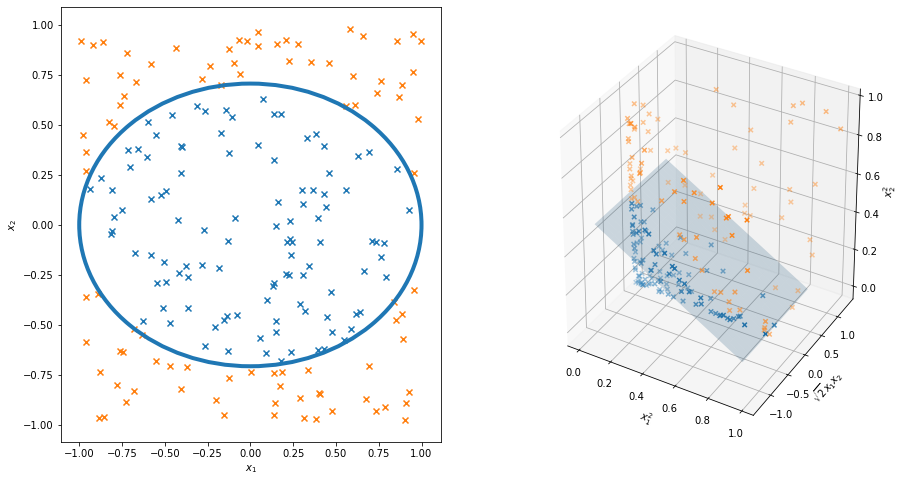
\includegraphics[width=0.9\linewidth,height=0.2\textheight,keepaspectratio]{Figure-23-01}
\end{figure}

There is a potential drawback. If we significantly expand the dimension
of the problem, we might increase the computational burden. For example,
if \(x\) has dimension \(d = 256\) and we wanted to use all fourth order
terms, then \(z = \phi(x)\) has dimension 183,181,376. What saves us is
two observations. First, many classifiers do not require that we know
the values of the individual points but, rather, just the inner product
between pairs of points. Second, notice in our example that the inner
product in \(\mathcal{Z}\) can be written

\[ 
\begin{align}
\langle z, \tilde{z} \rangle &= \langle \phi(x), \phi(\tilde{x}) \rangle \\
&= x_1^2 \tilde{x}_1^2 + 2 x_1 \tilde{x_1} x_2 \tilde{x}_2 + x_2^2 \tilde{x}_2^2 \\
&= ( \langle x, \tilde{x} \rangle )^2 \\
&\equiv K(x, \tilde{x})
\end{align}
\]

Thus, we can compute \(\langle z, \tilde{z} \rangle\) without ever
computing \(Z_i = \phi(X_i)\).

To summarize, kernelization means finding a mapping
\(\phi: \mathcal{X} \rightarrow \mathcal{Z}\) such that:

\begin{enumerate}
\def\labelenumi{\arabic{enumi}.}
\item
  \(\mathcal{Z}\) has higher dimension that \(\mathcal{X}\) and so leads
  to a richer set of classifiers.
\item
  The classifier only requires computing inner products.
\item
  There is a function \(K\), called a kernel, such that
  \(\langle \phi(x), \phi(\tilde{x}) \rangle = K(x, \tilde{x})\)
\end{enumerate}

Then, everywhere the term \(\langle x, \tilde{x} \rangle\) appears in
the algorithm, replace it with \(K(x, \tilde{x})\).

In fact, we never need to construct the mapping \(\phi\) at all. We only
need to specify a kernel \(K(x, \tilde{x})\) that corresponds to
\(\langle \phi(x), \phi(\tilde{x}) \rangle\) for some \(\phi\). This
raises an interesting question: given a function of two variables
\(K(x, y)\), does exist a function \(\phi(x)\) such that
\(K(x, y) = \langle \phi(x), \phi(\tilde{x}) \rangle\) ? The answer is
provided by \textbf{Mercer's theorem} which says, roughly, that if \(K\)
is positive definite -- meaning that

\[ \int \int K(x, y) f(x) f(y) dx dy \geq 0 \]

for square integrable functions \(f\) -- then such a \(\phi\) exists.
Examples of commonly used kernels are:

\begin{itemize}[tightlist]
\item
  polynomial: \(K(x, \tilde{x}) = (\langle x, \tilde{x} \rangle + a)^r\)
\item
  sigmoid:
  \(K(x, \tilde{x}) = \text{tanh} (a \langle x, \tilde{x} \rangle + b)\)
\item
  Gaussian:
  \(K(x, \tilde{x}) = -\exp \left( - \Vert x - \tilde{x} \Vert^2 / (2 \sigma^2) \right)\)
\end{itemize}

Let us now see how we can use this trick in LDA and in support vector
machines.

Recall that the Fisher linear discriminant method replaces \(X\) with
\(U = w^T X\) where \(w\) is chosen to maximize the Rayleigh coefficient

\[ J(w) = \frac{w^T S_B w}{w^T S_W w} \]

where

\[ S_B = (\overline{X}_0 - \overline{X}_1)(\overline{X}_0 - \overline{X}_1)^T \]

and

\[ S_W = \left( \frac{(n_0 - 1) S_0}{(n_0 - 1) + (n_1 - 1)} \right) + \left( \frac{(n_1 - 1) S_1}{(n_0 - 1) + (n_1 - 1)} \right) \]

In the kernelized version, we replace \(X_i\) with \(Z_i = \phi(X_i)\)
and find \(w\) to maximize

\[ J(w) = \frac{w^T S_B w}{w^T S_W w} \]

where

\[ S_B = (\overline{Z}_0 - \overline{Z}_1)(\overline{Z}_0 - \overline{Z}_1)^T \]

and

\[ S_W = \left( \frac{(n_0 - 1) \tilde{S}_0}{(n_0 - 1) + (n_1 - 1)} \right) + \left( \frac{(n_1 - 1) \tilde{S}_1}{(n_0 - 1) + (n_1 - 1)} \right) \]

Here, \(\tilde{S}_j\) is the sample covariance of the \(Z_i\)'s for
which \(Y_i = j\). However, to take advantage of kernelization, we need
to reexpress this in terms of inner products and then replace the inner
products with kernels.

It can be shown that the maximizing vector \(w\) is a linear combination
of the \(Z_i\)'s. Then we can write

\[ w = \sum_{i=1}^n \alpha_i Z_i \]

Also,

\[ \overline{Z}_j = \frac{1}{n_j} \sum_{i=1}^n \phi(X_i) I(Y_i = j) \]

Therefore,

\[
\begin{align}
w^T \overline{Z}_j &= \left( \sum_{i=1}^n \alpha_i Z_i \right)^T \left( \frac{1}{n_j} \sum_{i=1}^n \phi(X_i) I(Y_i = j) \right) \\
&= \frac{1}{n_j} \sum_{i=1}^n \sum_{s=1}^n \alpha_i I(Y_s = j) Z_i^T Z_s \\
&= \frac{1}{n_j} \sum_{i=1}^n \alpha_i \sum_{s=1}^n I(Y_s = j) \phi(X_i)^T \phi(X_s) \\
&= \frac{1}{n_j} \sum_{i=1}^n \alpha_i \sum_{s=1}^n I(Y_s = j) K(X_i, X_s) \\
&= \alpha^T M_j
\end{align}
\]

where \(M_j\) is a vector whose \(i\)-th component is

\[ M_j(i) = \frac{1}{n_j} \sum_{s=1}^n K(X_i, X_s) I(Y_s = j) \]

It follows that

\[ w^T \tilde{S}_B w = \alpha^T M \alpha \]

where \(M = (M_0 - M_1)(M_0 - M_1)^T\). By similar calculations, we can
write

\[ w^T \tilde{S}_W w = \alpha^T N \alpha \]

where

\[ N = K_0\left( I - \frac{1}{n_0}\mathbf{1}\right) K_0^T + K_1\left( I - \frac{1}{n_1}\mathbf{1}\right) K_1^T\]

\(I\) is the identity matrix, \(\mathbf{1}\) is a matrix of all 1s, and
\(K_j\) is the \(n \times n_j\) matrix with entries
\((K_j)_{rs} = K(x_r, x_s)\) with \(x_s\) varying over the observations
in group \(j\). Hence, we now find \(\alpha\) to maximize

\[ J(\alpha) = \frac{\alpha^T M \alpha}{\alpha^T N \alpha} \]

Notice that all the quantities are expressed in terms of the kernel.
Formally, the solution is \(\alpha = N^{-1}(M_0 - M_1)\). However, \(N\)
might be non-invertible. In this case, one replaces \(N\) by \(N + bI\)
for some constant \(b\). Finally, the projection onto the new subspace
can be written as

\[ U = w^T \phi(x) = \sum_{i=1}^N \alpha_i K(x_i, x) \]

The support vector machine can be similarly kernelized. We simply
replace \(\langle X_i, X_j \rangle\) with \(K(X_i, X_j)\). The
hyperplane can be written as
\(\hat{H}(X) = \hat{\alpha}_0 + \sum_{i=1}^n \hat{\alpha}_i Y_i K(X, X_i)\).

\subsubsection{23.11 Other Classifiers}\label{other-classifiers}

There are many other classifiers and space precludes a full discussion
of them. Let us briefly mention a few.

The \textbf{k-nearest neighbors} classifier is very simple. Given a
point \(x\), find the \(k\) data points closest to \(x\). Classify \(x\)
using the majority vote of these \(k\) neighbors. Ties can be broken
randomly; the parameter \(k\) can be chosen by cross-validation.

\textbf{Bagging} is a method for reducing the variability of a
classifier. It is most helpful for highly non-linear classifiers such as
a tree. We draw \(B\) bootstrap samples from the data. The \(b\)-th
bootstrap sample yields a classifier \(h_b\). The final classifier is

\[ 
\hat{x} = \begin{cases}
1 & \text{if } \frac{1}{B} \sum_{b=1}^B h_b(x) \geq \frac{1}{2} \\
0 & \text{otherwise}
\end{cases}
\]

\textbf{Boosting} is a method for starting with a simple classifier and
gradually improving it by refitting the data giving higher weight to
misclassified samples. Suppose that \(\mathcal{H}\) is a collection of
classifiers, for example, trees with only one split. Assume that
\(Y_i \in \{ -1, 1 \}\) and that each tree classifier \(h\) is such that
\(h(x) \in \{ -1, 1 \}\). We usually give equal weight to all data
points in the methods we have discussed. But one can incorporate unequal
weights quite easily in most algorithms. For example, in constructing a
tree, we could replace the impurity measure with a weighted impurity
measure. The original version of boosting, called AdaBoost, is as
follows.

\begin{enumerate}
\def\labelenumi{\arabic{enumi}.}
\item
  Set the weights \(w_i = 1 / n\), \(i = 1, \dots, n\).
\item
  For \(j = 1, \dots, J\), do the following steps:

  \begin{enumerate}
  \def\labelenumii{(\alph{enumii})}
  \item
    Construct a classifier \(h_J\) from the data using weights
\(w_1, \dots, w_n\).
  \item
    Compute the weighted error estimate:
  \end{enumerate}

  \[ \hat{L}_j = \frac{\sum_{i=1}^n w_i I(Y_i \neq h_j(X_i) }{\sum_{i=1}^n w_i} \]

  \begin{enumerate}
  \def\labelenumii{(\alph{enumii})}
  \setcounter{enumii}{2}
  \item
    Let \(\alpha_j = \log (( 1 - \hat{L}_j) / \hat{L}_j)\)
  \item
    Update the weights:
  \end{enumerate}

  \[ w_i \leftarrow w_i e^{\alpha_j I(Y_i \neq h_j(X_i)} \]
\item
  The final classifier is

  \[ \hat{h}(x) = \text{sign} \left( \sum_{j=1}^J \alpha_j h_j(x) \right) \]
\end{enumerate}

There is an enormous literature trying to explain and improve on
boosting. Whereas bagging is a variance reduction technique, boosting
can be thought of as a bias reduction technique. We starting with a
simple -- and hence highly biased -- classifier, and we gradually reduce
the bias. The disadvantage of boosting is that the final classifier is
quite complicated.

\subsubsection{23.13 Exercises}\label{exercises}

\textbf{Exercise 23.13.1}. Prove Theorem 23.5.

The Bayes rule is optimal, that is, if \(h\) is any classification rule
then \(L(h^*) \leq L(h)\).

\textbf{Solution}. We have:

\[ 
L(h) - L(h^*) = \mathbb{P}(h(X) \neq Y) - \mathbb{P}(h^*(X) \neq Y) 
= \int_\mathcal{X} \left( \mathbb{P}(h(X) \neq Y | X = x) - \mathbb{P}(h^*(X) \neq Y | X = x) \right) d\mathbb{P}_X(x)
\]

We will show that the integrand is non-negative,

\[ \mathbb{P}(h(X) \neq Y | X = x) - \mathbb{P}(h^*(X) \neq Y | X = x) \geq 0 \]

For any classifier \(h\),

\[ 
\begin{align}
\mathbb{P}(h(X) \neq Y | X = x) &= \mathbb{P}(h(X) = 0, Y = 1 | X = x) + \mathbb{P}(h(X) = 1, Y = 0 | X = x) \\
&= I(h(x) = 0) \mathbb{P}(Y = 1 | X = x) + I(h(x) = 1) \mathbb{P}(Y = 0 | X = x) \\
&= I(h(x) = 0) r(x) + (1 - I(h(x) = 0)) (1 - r(x)) \\
&= I(h(x) = 0) (2 r(x) - 1) + (1 - r(x))
\end{align}
\]

where \(r(x) = \mathbb{E}(Y | X = x)\). We can then write:

\[ 
\begin{align}
&\mathbb{P}(h(X) \neq Y | X = x) - \mathbb{P}(h^*(X) \neq Y | X = x) \\
&= \left(I(h(x) = 0) (2 r(x) - 1) + (1 - r(x)) \right) - \left(I(h^*(x) = 0) (2 r(x) - 1) + (1 - r(x)) \right) \\
&= (2 r(x) - 1) \left( I(h(x) = 0) - I(h^*(x) = 0) \right)
\end{align}
\]

Now:

\begin{itemize}[tightlist]
\item
  If \(h(x) = h^*(x)\), the second term in this product is 0, so the
  integrand is zero (and thus non-negative).
\item
  If \(h(x) = 0\) and \(h^*(x) = 1\), then \(r(x) \geq 1/2\), so the
  integrand is non-negative.
\item
  If \(h(x)= 1\) and \(h^*(x) = 0\), then \(r(x) \leq 1/2\), so the
  integrand is non-negative.
\end{itemize}

Since the integrand is always non-negative, the integral is
non-negative, and \(L(h^*) \leq L(h)\).

\textbf{Exercise 23.13.2}. Prove Theorem 23.7.

If \(X | Y = 0 \sim N(\mu_0, \Sigma_0)\) and
\(X | Y = 1 \sim N(\mu_1, \Sigma_1)\), then the Bayes rule is

\[
h^*(x) = \begin{cases}
1 & \text{if } r_1^2 < r_0^2 + 2 \log \left( \frac{\pi_1}{\pi_0} \right) + \log \left( \frac{| \Sigma_0 | }{ | \Sigma_1| }
\right) \\
0 & \text{otherwise} 
\end{cases}
\]

where

\[ r_i^2 = (x - \mu_i)^T \Sigma_i^{-1}(x - \mu_i), \quad i = 1, 2 \]

is the \textbf{Manalahobis distance}. An equivalent way of expressing
Bayes' rule is

\[ h(x) = \text{argmax}_k \delta_k(x) \]

where

\[ \delta_k(x) = -\frac{1}{2} \log | \Sigma_k | - \frac{1}{2} (x - \mu_k)^T \Sigma_k^{-1} (x - \mu_k) + \log \pi_k \]

and \(|A|\) denotes the determinant of matrix \(A\).

\textbf{Solution}. The joint distribution of \(X, Y\) is:

\[
\begin{align}
f_{X, Y}(x, y) &= f_{X | Y}(x | y) f_Y(y) \\
&= \sum_j \left( (2 \pi)^{k / 2} |\Sigma_j|^{-1/2} \exp \left\{ -\frac{1}{2} (x - \mu_j)^T \Sigma_j^{-1} (x - \mu_j) \right\} \right) \left( I(y = j) \pi_j \right)
\end{align}
\]

so the distribution of \(Y | X\) is

\[
\begin{align}
f_{Y | X}(y | x) &= \frac{f_{X, Y}(x, y)}{f_X(x)} = \frac{f_{X, Y}(x, y)}{\sum_{y_j} f_{X, Y}(x, y_j)} \\
&= \frac{\sum_j I(y = j) \pi_j (2 \pi)^{k / 2} |\Sigma_j|^{-1/2} \exp \left\{ -\frac{1}{2} (x - \mu_j)^T \Sigma_j^{-1} (x - \mu_j) \right\}}{\sum_j \pi_j (2 \pi)^{k / 2} |\Sigma_j|^{-1/2} \exp \left\{ -\frac{1}{2} (x - \mu_j)^T \Sigma_j^{-1} (x - \mu_j) \right\}} \\
&= \frac{\sum_j I(y = j) \pi_j |\Sigma_j|^{-1/2} \exp \left\{ -\frac{1}{2} (x - \mu_j)^T \Sigma_j^{-1} (x - \mu_j) \right\}}{\sum_j \pi_j |\Sigma_j|^{-1/2} \exp \left\{ -\frac{1}{2} (x - \mu_j)^T \Sigma_j^{-1} (x - \mu_j) \right\}}
\end{align}
\]

Let

\[ a_j(x) = \pi_j |\Sigma_j|^{-1/2} \exp \left\{ -\frac{1}{2} (x - \mu_j)^T \Sigma_j^{-1} (x - \mu_j) \right\} \]

Then we can write:

\[
f_{Y | X}(y | x) = \frac{a_y(x)}{a_0(x) + a_1(x)}
\]

Now,

\[ r(x) = \mathbb{E}[Y | X = x] = \sum_{y \in \mathcal{Y}} y \mathbb{P}(Y = y | X = x) = \mathbb{P}(Y = 1 | X = x) = \frac{a_1(x)}{a_0(x) + a_1(x)}\]

so \(r(x) > \frac{1}{2}\) is equivalent to \(a_1(x) > a_0(x)\), or

\[
\begin{align}
\pi_1 |\Sigma_1|^{-1/2} \exp \left\{ -\frac{1}{2} (x - \mu_1)^T \Sigma_1^{-1} (x - \mu_1) \right\}
&>
\pi_0 |\Sigma_0|^{-1/2} \exp \left\{ -\frac{1}{2} (x - \mu_1)^T \Sigma_0^{-1} (x - \mu_0) \right\} \\
\log \pi_1 - \frac{1}{2} \log |\Sigma_1| - \frac{1}{2} r_1^2
&>
\log \pi_0 - \frac{1}{2} \log |\Sigma_0| -\frac{1}{2} r_0^2 \\
r_1^2 &< r_0^2 + 2 \log \left( \frac{\pi_1}{\pi_0} \right) + \log \left( \frac{| \Sigma_0 | }{ | \Sigma_1| }
\right)
\end{align}
\]

which is the desired result. The inequalities above also show that the
two formulations of the rule are equivalent.

\textbf{Exercise 23.13.3}. Download the spam data from:

http://www-stat.stanford.edu/\textasciitilde tibs/ElemStatLearn/index.htm

The data file can also be found on the course web page. The data contain
57 covariates relating to email messages. Each email message was
classified as spam (Y=1) or not spam (Y=0). The outcome Y is the last
column in the file. The goal is to predict whether an email is spam or
not.

\textbf{(a)} Construct classification rules using (i) LDA, (ii) QDA,
(iii) logistic regression and (iv) a classification tree. For each,
report the observed misclassification error rate and construct a 2-by-2
table of the form

\[
\begin{array}{c|cc}
 & \hat{h}(x) = 0 & \hat{h}(x) = 1 \\
\hline
Y = 0 \\
Y = 1
\end{array}
\]

\textbf{(b)} Use 5-fold cross-validation to estimate the prediction
accuracy of LDA and logistic regression.

\textbf{(c)} Sometimes it helps to reduce the number of covariates. One
strategy is to compare \(X_i\) for the spam and email group. For each of
the 57 covariates, test whether the mean of the covariate is the same or
different between the two groups. Keep the 10 covariates with the
smallest p-values. Try LDA and logistic regression using only these 10
variables.

\textbf{Solution}.

\begin{python}
import numpy as np
import pandas as pd

data = pd.read_csv('data/spam.txt', header=None, delim_whitespace=True)
X, Y = data.loc[:, data.columns != 57].to_numpy(), data.loc[:, 57].to_numpy()
\end{python}

\textbf{(a)}

\begin{python}
def run_classifier(classifier, X, Y):
    classifier.fit(X, Y)
    Y_pred = classifier.predict(X)
    n = len(Y)
    
    true_positives = np.sum((Y_pred == 1) & (Y == 1))
    false_positives = np.sum((Y_pred == 1) & (Y == 0))
    false_negatives = np.sum((Y_pred == 0) & (Y == 1))
    true_negatives = np.sum((Y_pred == 0) & (Y == 0))

    return {
        'misclassification_rate': (false_positives + false_negatives) / n,
        'confusion_matrix': np.array([[true_positives, false_positives], [false_negatives, true_negatives]])
    }

def print_results(classifier_name, results):
    print('%s misclassification rate: %.3f' % (classifier_name, results['misclassification_rate']))
    print('%s confusion matrix:' % classifier_name)
    print(results['confusion_matrix'])
\end{python}

\begin{python}
from sklearn.discriminant_analysis import LinearDiscriminantAnalysis

classifier_name = 'LDA'
classifier = LinearDiscriminantAnalysis()
results = run_classifier(classifier, X, Y)
print_results(classifier_name, results)
\end{python}

\begin{console}
LDA misclassification rate: 0.111
LDA confusion matrix:
[[1426  125]
 [ 387 2663]]
\end{console}

\begin{python}
from sklearn.discriminant_analysis import QuadraticDiscriminantAnalysis

classifier_name = 'QDA'
classifier = QuadraticDiscriminantAnalysis()
results = run_classifier(classifier, X, Y)
print_results(classifier_name, results)
\end{python}

\begin{console}
QDA misclassification rate: 0.167
QDA confusion matrix:
[[1731  687]
 [  82 2101]]
\end{console}

\begin{python}
from sklearn.linear_model import LogisticRegression

classifier_name = 'Logistic Regression'
classifier = LogisticRegression(max_iter=2000, random_state=0)
results = run_classifier(classifier, X, Y)
print_results(classifier_name, results)
\end{python}

\begin{console}
Logistic Regression misclassification rate: 0.068
Logistic Regression confusion matrix:
[[1623  122]
 [ 190 2666]]
\end{console}

\begin{python}
from sklearn.tree import DecisionTreeClassifier

classifier_name = 'Decision Tree Classifier'
classifier = DecisionTreeClassifier(random_state=0)
results = run_classifier(classifier, X, Y)
print_results(classifier_name, results)
\end{python}

\begin{console}
Decision Tree Classifier misclassification rate: 0.001
Decision Tree Classifier confusion matrix:
[[1810    0]
 [   3 2788]]
\end{console}

\textbf{(b)}

\begin{python}
from sklearn.model_selection import KFold

def run_classifier_kfold(classifier, X, Y, n_splits=5):
    kf = KFold(n_splits=n_splits, shuffle=False)
    accuracy = np.empty(n_splits)
    for i, (train_index, test_index) in enumerate(kf.split(X)):
        classifier.fit(X[train_index], Y[train_index])
        Y_pred = classifier.predict(X[test_index])
        accuracy[i] = np.sum(Y_pred == Y[test_index]) / len(Y_pred)
    
    return accuracy.mean()
\end{python}

\begin{python}
classifier_name = 'LDA'
classifier = LinearDiscriminantAnalysis()

accuracy = run_classifier_kfold(classifier, X, Y, n_splits=5)

print('%s accuracy (5-fold): %.3f' % (classifier_name, accuracy))
\end{python}

\begin{console}
LDA accuracy (5-fold): 0.816
\end{console}

\begin{python}
classifier_name = 'Logistic Regression'
classifier = LogisticRegression(max_iter=2000, random_state=0)

accuracy = run_classifier_kfold(classifier, X, Y, n_splits=5)

print('%s accuracy (5-fold): %.3f' % (classifier_name, accuracy))
\end{python}

\begin{console}
Logistic Regression accuracy (5-fold): 0.859
\end{console}

\textbf{(c)}

\begin{python}
from scipy.stats import ttest_ind

X0 = X[Y == 0]
X1 = X[Y == 1]

num_features = X.shape[1]
num_selected = 10

pvalues = np.empty(num_features)

for k in range(num_features):
    _, pvalues[k] = ttest_ind(X0[:, k], X1[:, k])
    
selected_features = np.argpartition(pvalues, num_selected)[:num_selected]

X_filtered = X[:, selected_features]
\end{python}

\begin{python}
from sklearn.discriminant_analysis import LinearDiscriminantAnalysis

classifier_name = 'LDA'
classifier = LinearDiscriminantAnalysis()
results = run_classifier(classifier, X_filtered, Y)
print_results(classifier_name, results)
\end{python}

\begin{console}
LDA misclassification rate: 0.159
LDA confusion matrix:
[[1229  149]
 [ 584 2639]]
\end{console}

\begin{python}
from sklearn.linear_model import LogisticRegression

classifier_name = 'Logistic Regression'
classifier = LogisticRegression(max_iter=2000, random_state=0)
results = run_classifier(classifier, X_filtered, Y)
print_results(classifier_name, results)
\end{python}

\begin{console}
Logistic Regression misclassification rate: 0.121
Logistic Regression confusion matrix:
[[1413  156]
 [ 400 2632]]
\end{console}

\begin{python}
classifier_name = 'LDA'
classifier = LinearDiscriminantAnalysis()

accuracy = run_classifier_kfold(classifier, X_filtered, Y, n_splits=5)

print('%s accuracy (5-fold): %.3f' % (classifier_name, accuracy))
\end{python}

\begin{console}
LDA accuracy (5-fold): 0.780
\end{console}

\begin{python}
classifier_name = 'Logistic Regression'
classifier = LogisticRegression(max_iter=2000, random_state=0)

accuracy = run_classifier_kfold(classifier, X_filtered, Y, n_splits=5)

print('%s accuracy (5-fold): %.3f' % (classifier_name, accuracy))
\end{python}

\begin{console}
Logistic Regression accuracy (5-fold): 0.817
\end{console}

\textbf{Exercise 23.13.4}. Let \(\mathcal{A}\) be the set of
two-dimensional spheres. That is, \(A \in \mathcal{A}\) if
\(A = \{ (x, y) : (x - a)^2 + (y - b)^2 \leq c \}\) for some
\(a, b, c\). Find the VC dimension of \(\mathcal{A}\).

\textbf{Solution}. The VC dimension is 3.

Note that \(\mathcal{A}\) shatters any set of 3 non-collinear points in
a plane:

\begin{itemize}[tightlist]
\item
  A sufficiently small circle centered at any point will select just it,
  so we can always separate sets of size 1.
\item
  For separating a set of size 2, consider all circles with center \(C\)
  equidistant from points \(X\) and \(Y\), on the half plane that does
  not contain \(Z\). Any circle with radius \(r\) such that
  \(|CZ| > r > |CX| = |CY|\) will separate \(\{ X, Y \}\) from \(Z\).
  Note that for sufficiently far away center \(C\) this will be the
  case, since \(|CX| = |CY|\) converges monotonically to
  \(|C\overline{X}|\) and \(|CZ|\) converges monotonically to
  \(|C\overline{Z}|\), where \(\overline{Q}\) is the projection of point
  \(Q\) on the line containing the centers / the line equidistant from
  \(X\) and \(Y\). Since \(|C\overline{X}| < |C\overline{Z}|\), such
  circles must exist.
\end{itemize}

For 4 points, note that:

\begin{itemize}[tightlist]
\item
  If the 4 points are not in a convex hull, they cannot be shattered by
  \(\mathcal{A}\): any circle containing the 3 outermost points will
  need to contain all points inside the triangle set by them, so it will
  also need to contain the fourth point.
\item
  If the 4 points are in a convex hull, they form a convex
  quadrilateral. Let the points be \(X, Y, Z, W\), and assume without
  loss of generality that \(\angle X + \angle Z \leq 180^\circ\). Note
  that there is no circle that contains \(X, Z\) but not \(Y\) nor
  \(W\): we can reduce the radius of the circle and shift its center
  until \(X\) and \(Y\) are on its circumference. Assuming that both
  \(Y\) and \(W\) are outside of the circle implies that
  \(\angle Y + \angle W < 180^\circ\), which is a contradiction with the
  quadrilateral being convex.
\end{itemize}

Yet another argument can be build based on the fact that the VC
dimension of half-planes is also 3: Assume there is a set of 4 points
\(U\) that can be shattered by circles. Then for any set
\(S \subset U\), there exists a circle \(C\) such that \(C \cap U = S\)
and a circle \(C'\) such that \(C' \cap U = U \setminus S\). Therefore,
\(C \cap C'\) contains no points of \(U\). If \(C \cap C' = \emptyset\),
\(C\) and \(C'\) can be separated by a line. Otherwise, there is a line
that passes through the intersection of \(C\) and \(C'\), and it
separates \(S\) from \(U \setminus S\). This implies that \(U\) can be
shattered by half-planes, a contradiction.

Reference for second argument:
https://cstheory.stackexchange.com/a/11089 (applied to spheres and
half-spaces in \(\mathbb{R}^3\), instead of circles and half-planes in
\(\mathbb{R}^2\))

\textbf{Exercise 23.13.5}. Classify the spam data using support vector
machines.

\emph{(instructions on using SVM software for R omitted)}

\textbf{Solution}.

\begin{python}
import numpy as np
import pandas as pd

data = pd.read_csv('data/spam.txt', header=None, delim_whitespace=True)
X, Y = data.loc[:, data.columns != 57].to_numpy(), data.loc[:, 57].to_numpy()
\end{python}

\begin{python}
def run_classifier(classifier, X, Y):
    classifier.fit(X, Y)
    Y_pred = classifier.predict(X)
    n = len(Y)
    
    true_positives = np.sum((Y_pred == 1) & (Y == 1))
    false_positives = np.sum((Y_pred == 1) & (Y == 0))
    false_negatives = np.sum((Y_pred == 0) & (Y == 1))
    true_negatives = np.sum((Y_pred == 0) & (Y == 0))

    return {
        'misclassification_rate': (false_positives + false_negatives) / n,
        'confusion_matrix': np.array([[true_positives, false_positives], [false_negatives, true_negatives]])
    }

def print_results(classifier_name, results):
    print('%s misclassification rate: %.3f' % (classifier_name, results['misclassification_rate']))
    print('%s confusion matrix:' % classifier_name)
    print(results['confusion_matrix'])
\end{python}

\begin{python}
from sklearn.svm import LinearSVC
from sklearn.preprocessing import StandardScaler

classifier_name = 'SVC'
classifier = LinearSVC(max_iter=100000, random_state=0)
results = run_classifier(classifier, StandardScaler().fit_transform(X), Y)
print_results(classifier_name, results)
\end{python}

\begin{console}
SVC misclassification rate: 0.073
SVC confusion matrix:
[[1603  124]
 [ 210 2664]]
\end{console}

\textbf{Exercise 23.13.6}. Use VC theory to get a confidence interval on
the true error rate of the LDA classifier in question 3. Suppose that
the covariate \(X = (X_1, \dots, X_d)\) has \(d\) dimensions. Assume
that each variable has a continuous distribution.

\textbf{Solution}. Using Theorem 23.19, a \(1 - \alpha\) confidence
interval for \(L(\hat{h})\) is \(\hat{L}_n(\hat{h}) \pm \epsilon_n\)
where

\[ \epsilon_n^2 = \frac{32}{n} \log \left( \frac{8 s(\mathcal{H}, n)}{\alpha} \right) \]

From theorem 23.21, and assuming the VC dimension is \(v = d\),

\[ s(\mathcal{H}, n) \leq n^d + 1 \]

This gives us

\[ \epsilon_n^2 \leq \frac{32}{n} \log \left( \frac{8 (n^d + 1)}{\alpha} \right) \approx \frac{32}{n} \left( \log \left( \frac{8}{\alpha} \right) + d \log n\right) \]

\begin{python}
import numpy as np
import pandas as pd

data = pd.read_csv('data/spam.txt', header=None, delim_whitespace=True)
X, Y = data.loc[:, data.columns != 57].to_numpy(), data.loc[:, 57].to_numpy()
\end{python}

\begin{python}
n, d = X.shape
alpha = 0.05
\end{python}

\begin{python}
epsilon = np.sqrt((np.log(8 / alpha) + d * np.log(n)) * 32 / n)
print(epsilon)
\end{python}

\begin{console}
1.8381639894860362
\end{console}

\ldots{} which is as large as to be useless, since we already know that
the loss function is bound between 0 and 1.

If instead we limit ourselves to only 10 dimensions,

\begin{python}
epsilon = np.sqrt((np.log(8 / alpha) + 10 * np.log(n)) * 32 / n)
print(epsilon)
\end{python}

\begin{console}
0.7885971226771238
\end{console}

\ldots{} which is still rather large, but at least it doesn't cover the
whole interval. Given the initial error rate estimate of
\(L(\hat{h}) = 0.159\), this gives a 95\% confidence interval of
\([0, .947)\).

\textbf{Exercise 23.13.7}. Suppose that \(X_i \in \mathbb{R}\) and that
\(Y_i = 1\) whenever \(|X_i| \leq 1\) and \(Y_i = 0\) whenever
\(|X_i| > 1\). Show that no linear classifier can perfectly classify
these data. Show that the kernelized data \(Z_i = (X_i, X_i^2)\) can be
linearly separated.

\textbf{Solution}. No linear classifier can perfectly classify this
data; any linear classifier in 1 dimension will be of the form
\(h(x) = I(x \geq c)\), \(h(x) = I(x > c)\), \(h(x) = I(x \leq c)\), or
\(h(x) = I(x < c)\) for some constant \(c\). Therefore, whenever
\(|X_i| > \max \{ 1, c \}\), \(Y_i = 1\), but the classifier will
necessarily mark the positive and the negative \(X_i\)s with distinct
labels.

The kernelized data can be trivially separated: use
\(h(x_1, x_2) = I(x_2 \leq 1)\). Due to the mapping
\(\phi(x) = (x, x^2)\), \(x_2 = x^2\), so \(|X_i| \leq 1\) if and only
if \(Z_{i2} = X_i^2 \leq 1\).

\textbf{Exercise 23.13.8}. Repeat question 5 using the kernel
\(K(x, \tilde{x}) = (1 + x^T\tilde{x})^p\). Choose \(p\) by
cross-validation.

\textbf{Solution}.

\begin{python}
import numpy as np
import pandas as pd

data = pd.read_csv('data/spam.txt', header=None, delim_whitespace=True)
X, Y = data.loc[:, data.columns != 57].to_numpy(), data.loc[:, 57].to_numpy()
\end{python}

\begin{python}
from sklearn.model_selection import KFold

def run_classifier_kfold(classifier, X, Y, n_splits=5):
    kf = KFold(n_splits=n_splits, shuffle=False)
    accuracy = np.empty(n_splits)
    for i, (train_index, test_index) in enumerate(kf.split(X)):
        classifier.fit(X[train_index], Y[train_index])
        Y_pred = classifier.predict(X[test_index])
        accuracy[i] = np.sum(Y_pred == Y[test_index]) / len(Y_pred)
    
    return accuracy.mean()
\end{python}

\begin{python}
# Custom kernel, K(x, y) = (1 + x^T y)^p
def p_kernel(p):
    def f(x, y):
        # Help numpy handle fractional powers for negative numbers
        a = (1 + x @ y.T)
        return np.sign(a) * (np.abs(a))**p
        
    return f
\end{python}

\begin{python}
from sklearn.svm import SVC
from sklearn.preprocessing import StandardScaler

# Pre-scale data to assist SVC
X_scaled = StandardScaler().fit_transform(X)

# Compute accuracy based on cross-validation for a given p
def get_accuracy(p):
    classifier = SVC(kernel=p_kernel(p), max_iter=1000000, random_state=0)
    return run_classifier_kfold(classifier, X_scaled, Y, n_splits=5)
\end{python}

\begin{python}
from tqdm import tqdm_notebook

accuracy_results = {}

step = 0.1
for p in tqdm_notebook(np.arange(-3, 3 + step, step=step)):
    accuracy_results[p] = get_accuracy(p)
    
accuracy_results = np.array([(a, b) for a, b in accuracy_results.items()]).T
\end{python}

\begin{python}
import matplotlib.pyplot as plt
%matplotlib inline

plt.figure(figsize=(12, 8))
plt.plot(accuracy_results[0], accuracy_results[1])
plt.xlabel('p')
plt.ylabel('Accuracy')
plt.show()

selected_index = np.argmax(accuracy_results[1])
selected_p = accuracy_results[0, selected_index]
selected_accuracy = accuracy_results[1, selected_index]
print('Selected hyperparameter p: %.1f' % selected_p)
print('Cross-validation accuracy: %.3f' % selected_accuracy)
\end{python}

\begin{figure}[H]
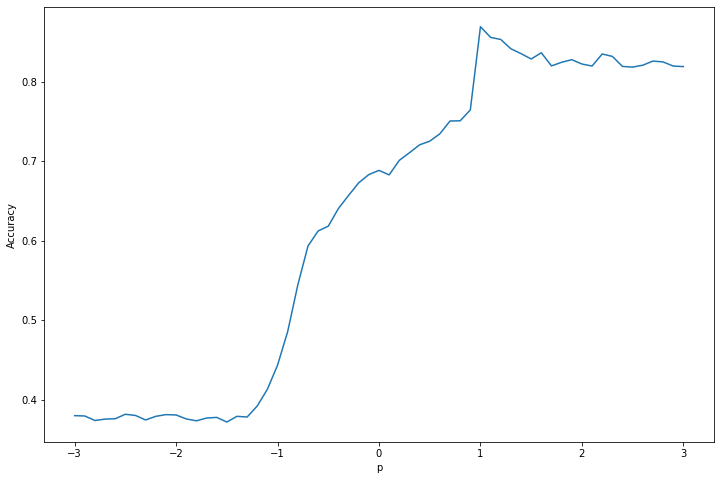
\includegraphics[width=0.9\linewidth,height=0.2\textheight,keepaspectratio]{Figure-23-02}
\end{figure}

\begin{console}
Selected hyperparameter p: 1.0
Cross-validation accuracy: 0.869
\end{console}

\textbf{Exercise 23.13.9}. Apply the \(k\)-nearest neighbors classifier
to the ``iris data''. Get the data in R from the command
\texttt{data(iris)}. Choose k by cross-validation.

\textbf{Solution}.

\begin{python}
# Load data from Python scikit-learn
from sklearn import datasets

iris = datasets.load_iris()
X, Y = iris.data, iris.target
\end{python}

\begin{python}
from sklearn.model_selection import KFold

def run_classifier_kfold(classifier, X, Y, n_splits=5):
    kf = KFold(n_splits=n_splits, shuffle=False)
    accuracy = np.empty(n_splits)
    for i, (train_index, test_index) in enumerate(kf.split(X)):
        classifier.fit(X[train_index], Y[train_index])
        Y_pred = classifier.predict(X[test_index])
        accuracy[i] = np.sum(Y_pred == Y[test_index]) / len(Y_pred)
    
    return accuracy.mean()
\end{python}

\begin{python}
from sklearn.neighbors import KNeighborsClassifier
from sklearn.preprocessing import StandardScaler

# Pre-scale data to assist classifier
X_scaled = StandardScaler().fit_transform(X)

# Compute accuracy based on cross-validation for a given p
def get_accuracy(k):
    classifier = KNeighborsClassifier(n_neighbors=k)
    return run_classifier_kfold(classifier, X_scaled, Y, n_splits=5)
\end{python}

\begin{python}
from tqdm import tqdm_notebook

accuracy_results = {}

for k in tqdm_notebook(range(1, 121)):
    accuracy_results[k] = get_accuracy(k)
    
accuracy_results = np.array([(a, b) for a, b in accuracy_results.items()]).T
\end{python}

\begin{python}
import matplotlib.pyplot as plt
%matplotlib inline

plt.figure(figsize=(12, 8))
plt.plot(accuracy_results[0], accuracy_results[1])
plt.xlabel('k')
plt.ylabel('Accuracy')
plt.show()

selected_index = np.argmax(accuracy_results[1])
selected_k = accuracy_results[0, selected_index]
selected_accuracy = accuracy_results[1, selected_index]
print('Selected hyperparameter k: %i' % selected_k)
print('Cross-validation accuracy: %.3f' % selected_accuracy)
\end{python}

\begin{figure}[H]
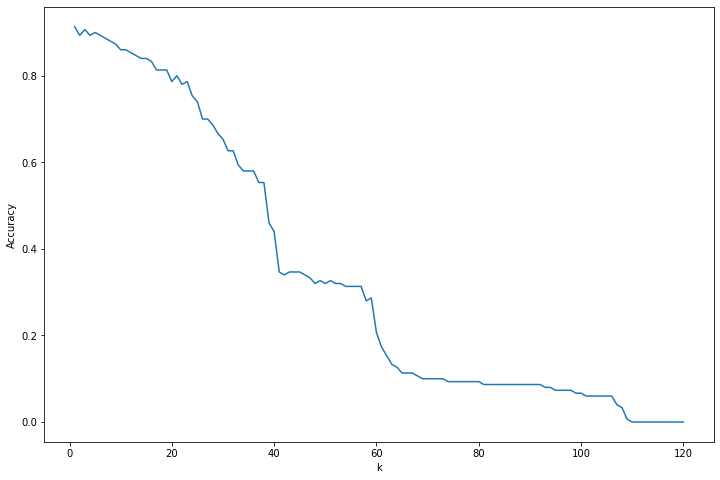
\includegraphics[width=0.9\linewidth,height=0.2\textheight,keepaspectratio]{Figure-23-03}
\end{figure}

\begin{console}
Selected hyperparameter k: 1
Cross-validation accuracy: 0.913
\end{console}

\textbf{Exercise 21.13.10 (Curse of Dimensionality)}. Suppose that \(X\)
has a uniform distribution on the \(d\)-dimensional cube
\([-1/2, 1/2]^d\). Let \(R\) be the distance from the origin to the
closest neighbor. Show that the median of \(R\) is

\[ \left( \frac{1 - \left(\frac{1}{2}\right)^{1/n}}{v_d(1)} \right)^{1/d}\]

where

\[ v_d(r) = r^d \frac{\pi^{d/2}}{\Gamma((d/2) + 1)} \]

is the volume of a sphere of radius \(r\). When does \(R\) exceed the
edge of the cube when \(n = 100, 1000, 10000\)?

\textbf{Solution}.

The probability that \(R\) is greater than or equal to some variable
\(x\) is the probability that all \(X_i\) are at a distance greater than
to \(x\) from the origin,

\[
\begin{align}
\mathbb{P}(R > x) &= \mathbb{P}(\{ d(X_i, 0) > x : i = 1, \dots, n \}) \\
&= \prod_{i=1}^n \mathbb{P}( d(X_i, 0) > x  ) \\
&= \prod_{i=1}^n \mathbb{P}\left( \sum_{j=1}^d X_{ij}^2 > x^2  \right) \\
&= \prod_{i=1}^n \int \int \dots \int I \left( \sum_{j=1}^d x_{ij}^2 > x^2 \right) dx_{i1} dx_{i2} \dots dx_{id} \\
&= \prod_{i=1}^n (1 - v_d(x)) \\
&= \left(1 - v_d(1) x^d\right)^n
\end{align}
\]

since the integral above represents the area in the \(d\)-dimensional
cube outside of the hypersphere of radius \(x\) centered in the origin,
and the \(d\)-sphere of radius \(x\) has volume \(v_d(x) = v_d(1) x^d\).

This means that the cumulative distribution function for \(R\) is

\[F(x) = \mathbb{P}(R \leq x) = 1 - \mathbb{P}(R > x) = 1 - \left(1 - v_d(1) x^d\right)^n\]

The inverse cumulative distribution function, then, is obtained by
replacing \(F(x) = y\) and solving for \(x = F^{-1}(y)\):

\[ F^{-1}(y) = \left( \frac{1 - (1 - y)^{1/n}}{v_d(1)} \right)^{1/d} \]

The median value is \(F^{-1}(1/2)\), so the result follows,

\[ F^{-1}\left( \frac{1}{2} \right) = \left( \frac{1 - \left( \frac{1}{2} \right)^{1/n}}{v_d(1)} \right)^{1/d}\]

Let's also provide a proof for the volume formula, and for the surface
area formula (below).

\[ a_d(r) = r^d \frac{2 \pi^{(d + 1)/2}}{\Gamma \left( \frac{d + 1}{2}\right)}  \]

Multiple proofs are available at
https://en.wikipedia.org/wiki/Volume\_of\_an\_n-ball; in keeping with
the theme of this book, let's follow the proof using Gaussian integers.

Consider the density function in \(d\) dimensions:

\[ f(x_1, \dots, x_d) = \exp \left\{ -\frac{1}{2} \sum_{i=1}^d x_i^2 \right\} \]

This density function is proportional to the probability density
function of a multivariate Gaussian \(N(0, I_d)\) by a factor of
\((2 \pi)^{d/2}\) and a PDF integrates to 1, so its volume integral is

\[ \int_{\mathbb{R}^d} f dV = (2 \pi)^{d/2}\]

Computing the same integral in spherical coordinates, on the
\(\mathbb{S}^{d - 1}\) sphere of \(d - 1\) dimensions,

\[ \int_{\mathbb{R}^d} f dV = \int_0^\infty \int_{\mathbb{S}^{d - 1}} \exp \left\{ -\frac{1}{2} r^2 \right\} dA dr \]

Using the fact that the surface area is proportional to the radius to
the power of the dimension of its space,
\(a_{d-1}(r) = a_{d-1}(1) r^{d-1}\), we get:

\[ a_{d-1}(1) \int_0^\infty \exp \left\{ -\frac{1}{2} r^2 \right\} r^{d - 1} dr \]

Replacing \(t = r^2 / 2\) to clean up the exponent, we end up with

\[ a_{d-1}(1) 2^{\frac{d}{2} - 1} \int_0^\infty t^{\frac{d}{2} - 1} e^{-t}  dt = a_{d-1}(1) 2^{\frac{d}{2} - 1} \Gamma \left( \frac{d}{2} \right)\]

Therefore, equating this to \((2 \pi)^{d/2}\), we prove the area formula
for radius 1 and dimension \(d - 1\), from which the formula above for
the area follows:

\[ a_{d - 1}(1) = \frac{2 \pi^{d/2}}{\Gamma \left( \frac{d}{2}\right)} \Longrightarrow a_d(r) = r^d \frac{2 \pi^{(d + 1)/2}}{\Gamma \left( \frac{d + 1}{2}\right)} \]

Now, to get the volume for the \(d\)-dimensional ball, we integrate the
surface area of dimension \(d-1\) and radius \(R\), and use that
\(\Gamma(z + 1) = z \Gamma(z)\):

\[ v_d(R) = \int_0^R a_{d-1}(r) dr = \int_0^R \frac{2 \pi^{d/2}}{\Gamma \left( \frac{d}{2}\right)} r^{d - 1} dr = R^d \frac{2 \pi^{d / 2}}{d \Gamma \left( \frac{d}{2} \right) } = R^d \frac{\pi^{d/2}}{\Gamma\left(\frac{d}{2} + 1\right)} \]

which is the desired expression.

\(R\) exceeds the edge of the cube when \(R > 1/2\); this occurs with
probability \(1 - F(1/2) = \left(1 - v_d(1) (1/2)^d\right)^n\) -- which
is a function of \(d\) and \(n\). Let's plot the curves over \(n\) for a
few values of \(d\):

\begin{python}
import numpy as np
from scipy.special import gamma

def v(d):
    ''' Returns the d-volume of a d-sphere of radius 1. '''
    return np.pi**(d / 2) / gamma(d/2 + 1)

def F(x, d, n):
    return 1 - (1 - v(d) * x**d)**n
\end{python}

\begin{python}
import matplotlib.pyplot as plt
%matplotlib inline

nn = np.arange(1, 10001)
plt.figure(figsize=(14.5, 8))
for d in range(1, 17):
    plt.plot(nn, 1 - F(x=1/2, d=d, n=nn), label='d = %i' % d)

plt.xscale('log')
plt.xlabel('n')
plt.ylabel('Probability of R outside cube')
plt.legend()
plt.show()
\end{python}

\begin{figure}[H]
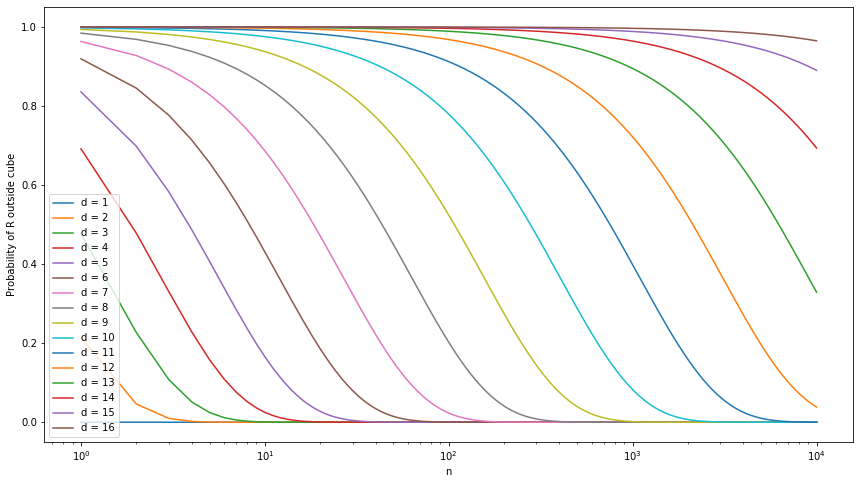
\includegraphics[width=0.9\linewidth,height=0.2\textheight,keepaspectratio]{Figure-23-04}
\end{figure}

Note that as \(d\) increases, it takes exponentially more samples to
have the probability of \(R\) staying inside the hypercube. This is the
case since the volume of the hyperball of radius 1 is exponential on
\(n\), using Stirling's approximation on the Gamma function:

\[ v_d(1) \approx \frac{1}{\sqrt{n \pi}} \left( \frac{2 \pi e}{n}\right)^{n/2} \]

\textbf{Exercise 23.13.11}. Fit a tree to the data in question 3. Now
apply bagging and report your results.

\textbf{Solution}.

We will use 5-fold cross-validation to select a number of base decision
tree classifiers to use in bagging.

\begin{python}
import numpy as np
import pandas as pd

data = pd.read_csv('data/spam.txt', header=None, delim_whitespace=True)
X, Y = data.loc[:, data.columns != 57].to_numpy(), data.loc[:, 57].to_numpy()
\end{python}

\begin{python}
from sklearn.model_selection import KFold

def run_classifier_kfold(classifier, X, Y, n_splits=5):
    kf = KFold(n_splits=n_splits, shuffle=False)
    accuracy = np.empty(n_splits)
    for i, (train_index, test_index) in enumerate(kf.split(X)):
        classifier.fit(X[train_index], Y[train_index])
        Y_pred = classifier.predict(X[test_index])
        accuracy[i] = np.sum(Y_pred == Y[test_index]) / len(Y_pred)
    
    return accuracy.mean()
\end{python}

\begin{python}
from sklearn.tree import DecisionTreeClassifier
from sklearn.ensemble import BaggingClassifier

def run_bagging_classifier(n_estimators):
    tree_classifier = DecisionTreeClassifier(random_state=0)
    bagging_classifier = BaggingClassifier(base_estimator=tree_classifier, n_estimators=n_estimators, random_state=0)
    return run_classifier_kfold(bagging_classifier, X, Y, n_splits=5)
\end{python}

\begin{python}
from tqdm import tqdm_notebook

accuracy_results = {}

for n_estimators in tqdm_notebook(range(1, 101)):
    accuracy_results[n_estimators] = run_bagging_classifier(n_estimators)
    
accuracy_results = np.array([(a, b) for a, b in accuracy_results.items()]).T
\end{python}

\begin{python}
import matplotlib.pyplot as plt

plt.figure(figsize=(12, 8))
plt.plot(accuracy_results[0], accuracy_results[1])
plt.xlabel('n_estimators')
plt.ylabel('Accuracy')
plt.show()

selected_index = np.argmax(accuracy_results[1])
selected_n = accuracy_results[0, selected_index]
selected_accuracy = accuracy_results[1, selected_index]
print('Selected hyperparameter n_estimators: %i' % selected_n)
print('Cross-validation accuracy: %.3f' % selected_accuracy)
\end{python}

\begin{figure}[H]
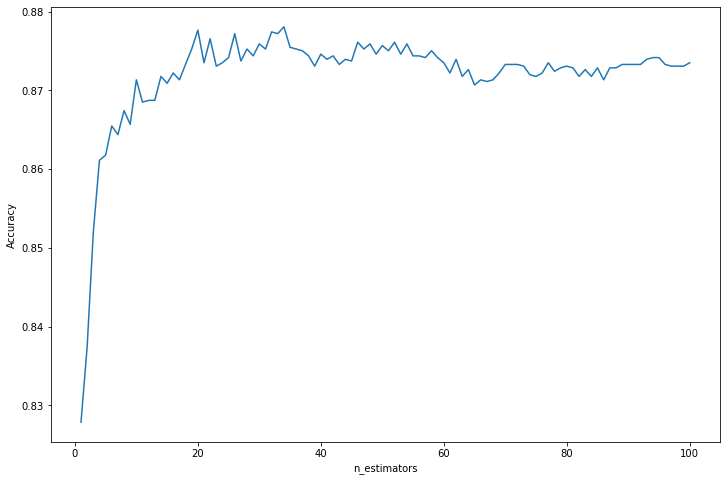
\includegraphics[width=0.9\linewidth,height=0.2\textheight,keepaspectratio]{Figure-23-05}
\end{figure}

\begin{console}
Selected hyperparameter n\_estimators: 34
Cross-validation accuracy: 0.878
\end{console}

\textbf{Exercise 23.13.12}. Fit a tree that uses only one split in one
variable to the data in question 3. Now apply boosting.

\textbf{Solution}.

\begin{python}
import numpy as np
import pandas as pd

data = pd.read_csv('data/spam.txt', header=None, delim_whitespace=True)
X, Y = data.loc[:, data.columns != 57].to_numpy(), data.loc[:, 57].to_numpy()
\end{python}

\begin{python}
from sklearn.model_selection import KFold

def run_classifier_kfold(classifier, X, Y, n_splits=5):
    kf = KFold(n_splits=n_splits, shuffle=False)
    accuracy = np.empty(n_splits)
    for i, (train_index, test_index) in enumerate(kf.split(X)):
        classifier.fit(X[train_index], Y[train_index])
        Y_pred = classifier.predict(X[test_index])
        accuracy[i] = np.sum(Y_pred == Y[test_index]) / len(Y_pred)
    
    return accuracy.mean()
\end{python}

\begin{python}
from sklearn.tree import DecisionTreeClassifier
from sklearn.ensemble import AdaBoostClassifier

def run_boosting_classifier(n_estimators):
    tree_classifier = DecisionTreeClassifier(max_depth=2, random_state=0)
    boosting_classifier = AdaBoostClassifier(base_estimator=tree_classifier, n_estimators=n_estimators, random_state=0)
    return run_classifier_kfold(boosting_classifier, X, Y, n_splits=5)
\end{python}

\begin{python}
from tqdm import tqdm_notebook

accuracy_results = {}

for n_estimators in tqdm_notebook(range(1, 101)):
    accuracy_results[n_estimators] = run_boosting_classifier(n_estimators)
    
accuracy_results = np.array([(a, b) for a, b in accuracy_results.items()]).T
\end{python}

\begin{python}
import matplotlib.pyplot as plt

plt.figure(figsize=(12, 8))
plt.plot(accuracy_results[0], accuracy_results[1])
plt.xlabel('n_estimators')
plt.ylabel('Accuracy')
plt.show()

selected_index = np.argmax(accuracy_results[1])
selected_n = accuracy_results[0, selected_index]
selected_accuracy = accuracy_results[1, selected_index]
print('Selected hyperparameter n_estimators: %i' % selected_n)
print('Cross-validation accuracy: %.3f' % selected_accuracy)
\end{python}

\begin{figure}[H]
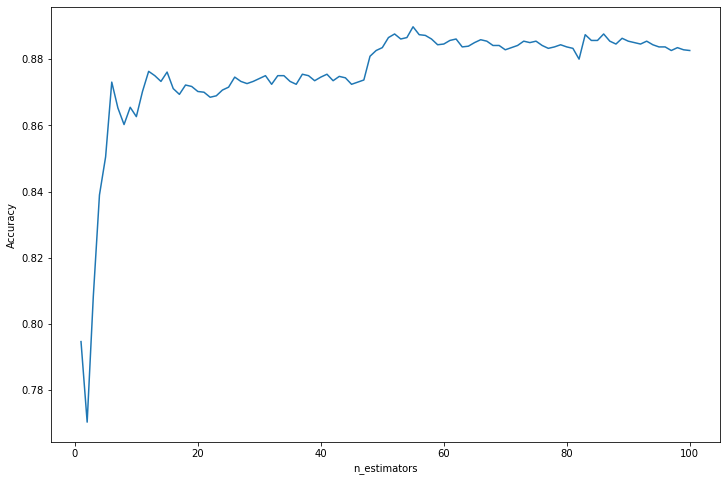
\includegraphics[width=0.9\linewidth,height=0.2\textheight,keepaspectratio]{Figure-23-06}
\end{figure}

\begin{console}
Selected hyperparameter n\_estimators: 55
Cross-validation accuracy: 0.890
\end{console}

\textbf{Exercise 23.13.13}. Let \(r(x) = \mathbb{P}(Y = 1 | X = x)\) and
let \(\hat{r}(x)\) be an estimate of \(r(x)\). Consider the classifier

\[
h(x) = \begin{cases}
1 &\text{if } \hat{r}(x) \geq 1/2 \\
0 &\text{otherwise}
\end{cases}
\]

Assume that \(\hat{r}(x) \approx N(\overline{r}(x), \sigma^2(x))\) for
some functions \(\overline{r}(x)\) and \(\sigma^2(x)\). Show that, for
fixed \(x\),

\[ \mathbb{P}(Y \neq h(x)) \approx \mathbb{P}(Y \neq h^*(x)) + 
\left| 2 r(x) - 1 \right| \times \left[ 1 - \Phi \left( \frac{\text{sign} \left( (r(x) - 1/2) (\overline{r}(x) - 1/2) \right)}{\sigma(x)} \right) \right]\]

where \(\Phi\) is the standard normal CDF and \(h^*\) is the Bayes rule.
Regard
\(\text{sign} \left( (r(x) - 1/2) (\overline{r}(x) - 1/2) \right)\) as a
type of bias term. Explain the implications for the bias-variance
trade-off in classification. (Friedman, 1997).

Hint: First show that

\[ \mathbb{P}(Y \neq h(x)) = |2 r(x) - 1| \mathbb{P}(h(x) \neq h^*(x)) + \mathbb{P}(Y \neq h^*(x))\]

\textbf{Solution}.

As in exercise 1, note that for any classifier \(h\),

\[ 
\begin{align}
\mathbb{P}(h(X) \neq Y | X = x) &= \mathbb{P}(h(X) = 0, Y = 1 | X = x) + \mathbb{P}(h(X) = 1, Y = 0 | X = x) \\
&= I(h(x) = 0) \mathbb{P}(Y = 1 | X = x) + I(h(x) = 1) \mathbb{P}(Y = 0 | X = x) \\
&= I(h(x) = 0) r(x) + (1 - I(h(x) = 0)) (1 - r(x)) \\
&= I(h(x) = 0) (2 r(x) - 1) + (1 - r(x))
\end{align}
\]

Then

\[
\mathbb{P}(Y \neq h(X) | X = x) - \mathbb{P}(Y \neq h^*(X) | X = x) = (2 r(x) - 1) \left(I(h(x) = 0) - I(h^*(x) = 0)\right)
\]

\begin{itemize}[tightlist]
\item
  When \(h(x) = h^*(x)\), the left term is zero, and the hint statement
  holds.
\item
  When \(h(x) = 1, h^*(x) = 0\), then \(r(x) \leq 1/2\) and
  \(I(h(x) = 0) - I(h^*(x) = 0) = -1\), so the hint statement holds.
\item
  When \(h(x) = 0, h^*(x) = 1\), then \(r(x) \geq 1/2\) and
  \(I(h(x) = 0) - I(h^*(x) = 0) = 1\), so the hint statement holds.
\end{itemize}

This proves the hint statement.

It now suffices to show that

\[ \mathbb{P}(h(x) \neq h^*(x)) \approx 1 - \Phi \left( \frac{\text{sign} \left( (r(x) - 1/2) (\overline{r}(x) - 1/2) \right)}{\sigma(x)} \right) \]

or its complement,

\[ \mathbb{P}(h(x) = h^*(x)) \approx \Phi \left( \frac{\text{sign} \left( (r(x) - 1/2) (\overline{r}(x) - 1/2) \right)}{\sigma(x)} \right) \]

But \(h(x)\) is a binomial variable, with

\[ \mathbb{P}(h(x) = 1) = \mathbb{P}\left(\hat{r}(x) \geq \frac{1}{2} \right) \approx \mathbb{P}\left( Z \geq \frac{\frac{1}{2} - \overline{r}(x)}{\sigma(x)} \right) = 1 - \Phi\left( \frac{\frac{1}{2} - \overline{r}(x)}{\sigma(x)} \right) = \Phi\left( \frac{\overline{r}(x) - \frac{1}{2}}{\sigma(x)} \right)\]

where \(Z \sim N(0, 1)\) and
\(\hat{r}(x) \approx N(\overline{r}(x), \sigma^2(x))\). Similarly,

\[ \mathbb{P}(h(x) = 0) \approx 1 - \Phi\left( \frac{\overline{r}(x) - \frac{1}{2}}{\sigma(x)} \right) = \Phi\left( \frac{\frac{1}{2} - \overline{r}(x)}{\sigma(x)} \right)\]

The result that follows applies the sign operator to the \textbf{first}
term in the product,

\[ \mathbb{P}(h(x) = h^*(x)) \approx \Phi \left( \frac{\text{sign} \Big\{ r(x) - 1/2 \Big\} (\overline{r}(x) - 1/2) }{\sigma(x)} \right) \]

I assume that the provided exercise meant this and has a typo.
Alternatively, take the poor approximation of moving the term outside of
the sign operator inside.

Implications for bias-variance tradeoff in classification are that both
better bias (\(\overline{r}(x)\) closer to \(r(x)\)) and smaller
variance lead to better bounds on the errors -- and the tradeoff for
this bound can be quantified by their ratio.

\textbf{\emph{Implementation note re: decision trees:}}
\emph{scikit-learn decision tree algorithms are good for API purposes,
but if you are looking to fit decision forests in larger problems
consider using a more specialized library, such as XGBoost or LightGBM,
with more modern algorithms and support for GPU. For much larger scale
problems, consider cloud-based machine learning providers, such as AWS's
Sagemaker or Google's ML Engine.}

\emph{Also consider more specific k-fold search strategies for problems
with imbalanced classes, such as stratified k-fold, and consider a more
formalized approach to hyperparameter search rather than an extensive
grid search.}
